%% Please see http://texdoc.net/pkg/ndsu-thesis for full documentation and options

%% phd,ms-thesis,ms-paper,ma-thesis,ma-paper
\documentclass{article}

%\title{Effects of User Interface in Communication Delays in Interplanetary Analog Missions}
\title{Bachelor Project}
\author{Christian Gommeringer}
% \authorpronound{his}
% \prevdega{Your Previous Degree \#1}
% \prevdegb{Your Previous Degree \#2}
% \gradmonth{August}
% \gradyear{2024}
% \department{Your Department}
% \cchair{Your committee chair}
% \cmembera{Your committee member \#1}
% \cmemberb{Your committee member \#2}
% \cmemberc{Your committee member \#3}
% \cmemberd{Your committee member \#4}
% \graddean{Name of Grad Dean}

% \abstract{Your abstract goes here. You can also use an input command with a filename.}
% \acknowledgements{Your acknowledgements go here. You can also use an input command with a filename.}
% \dedication{Your dedication goes here.}
\usepackage{amsmath}
\usepackage{amsfonts}
% \usepackage{unicode-math}
\usepackage{amssymb}
\usepackage{braket}
\usepackage{mathtools}
\usepackage[a4paper, margin=2cm]{geometry}
\usepackage{bbold}
\usepackage{graphicx}
\usepackage{wrapfig}
\usepackage{hyperref}
\usepackage{floatrow}
\usepackage{subcaption}
% \setmathfont{Asana Math}
% \makeglossaries
% \loadglsentries{glossary}

% Right align bibliography to get rid of under full warnings.
% There are two options for this. Preference is to keep bibliography justified. 
%\apptocmd{\thebibliography}{\raggedright}{}{}
% \apptocmd{\sloppy}{\hbadness 10000\relax}{}{}
% \overfullrule=5pt

\begin{document}
\newcommand{\half}{\frac{1}{2}}
\newcommand{\Tr}{\operatorname{Tr}}
\newcommand{\Trs}[1]{\Tr_S\left\{#1\right\}}
% \newcommand{\dt}[1]{\frac{\text{d} #1}{\text{d}t}}
\newcommand{\dt}{\frac{\text{d}}{\text{d}t}}
\newcommand{\tk}{\tilde{\kappa}}
\newcommand{\tw}{\tilde{\omega}}
\maketitle
\section*{Mean field considerations}
\subsection*{Deriving the ME from CM}
The system under examination is described in the CM formalism by the following Hamiltonian
\begin{align}\label{eq:Ham}
    H&=\left(\frac{\delta}{2}+\tilde{g}\,\alpha_z\right)\,J_z+\omega\,J_x+\tilde{g}\,\left(\alpha_x\,J_x\,\sigma_x+\alpha_y\,J_y\,\sigma_y+\alpha_z\,J_z\,\sigma_z\right)\notag\\
    \text{with}\quad{H_S}&\vcentcolon=\left(\frac{\delta}{2}+\tilde{g}\,\alpha_z\right)\,J_z+\omega\,J_x\\
    V_n\vcentcolon&=\tilde{g}\,\left(\alpha_x\,J_x\,\sigma_x+\alpha_y\,J_y\,\sigma_y+\alpha_z\,J_z\,\sigma_z\right)\quad.\notag
\end{align}
Here the $\alpha_i$ and $\delta$ are constant, whereas $\tilde{g}=g/\sqrt{\Delta{t}}$ has a time dependence of the time step we are now using to write the ME of this problem.
It is possible to formulate a discrete Lindblad Master Equation, following the description of \cite{overview}. The density matrix of the system evolves according to
\begin{align}\label{eq:ME}
\frac{\Delta \rho_n}{\Delta t} = -i[H_s + \operatorname{Tr}_\eta(V_n\,\eta_n), \rho_{n-1}] + \sum_{kk'} \left( L_{kk'} \rho_{n-1} L_{kk'}^\dagger - \frac{1}{2} \left[L_{kk'}^\dagger L_{kk'}, \rho_{n-1} \right]_+\right)
\end{align}
In this expression the spectral decomposition of the density matrix of the interacting ancilla is used
\begin{equation*}
    \eta=\sum_k\,p_k\,\ket{k}\bra{k}\quad,
\end{equation*}
in order to define the jump operators
\begin{equation*}
    L_{kk'}=\sqrt{p_k\,\Delta{t}}\,\braket{k'|V_n|k}\quad.
\end{equation*}
All ancillas are chosen to be in the ground state. Therefore the the density matrix of an ancilla takes the form
\begin{equation*}
    \eta=\left(\begin{array}{cc}
      0   & 0 \\
       0  & 1
    \end{array}\right)=\ket{\downarrow}\bra{\downarrow}
\end{equation*}
From this is inferred 
\begin{equation*}
    \operatorname{Tr}_\eta(V_n\,\eta_n)=-\tilde{g}\,\alpha_z\,J_z\quad,
\end{equation*}
and we can coalesce
\begin{align*}
    -i[H_s + \operatorname{Tr}_\eta(V_n\,\eta_n), \rho_{n-1}]=&-i[\delta/2\,J_z+\omega\,J_x,\rho_{n-1}]\\
    =&\vcentcolon-i[H_S',\rho_{n-1}]
\end{align*}
Since $p_\uparrow=0$, the only non-vanishing jump operators are
\begin{align*}
    L_{\downarrow\downarrow}&=\sqrt{\Delta{t}}\,\braket{\downarrow|V_n|\downarrow}\\
    &=-g\,\alpha_z\,J_z\\
    L_{\downarrow\uparrow}&=\sqrt{\Delta{t}}\,\braket{\uparrow|V_n|\downarrow}\\
    &={g}\,\left(\alpha_x\,J_x-i\,\alpha_y\,J_y\right)
\end{align*}
Plugging these findings into the terms of the ME\ref{eq:ME} yields
\begin{align*}
    \sum_{kk'} L_{kk'} \rho_{n-1} L_{kk'}^\dagger=&\sum_{k'} L_{\downarrow{k}'} \rho_{n-1} L_{\downarrow{k}'}^\dagger\\
    =&g^2\,\left(\alpha_z^2\,J_z\rho_{n-1}J_z^\dagger+(\alpha_x\,J_x-i\,\alpha_y\,J_y)\rho_{n-1}(\alpha_x\,J_x^\dagger+i\,\alpha_y\,J_y^\dagger)\right)\\
    =&g^2\,(\alpha_z^2\,J_z\rho_{n-1}J_z^\dagger+\alpha_y^2\,J_y\rho_{n-1}J_y^\dagger+\alpha_x^2\,J_x\rho_{n-1}J_x^\dagger\\
    &+i\,\alpha_x\,\alpha_y\,(J_x\rho_{n-1}J_y^\dagger-J_y\rho_{n-1}J_x^\dagger))\\\\
    \sum_{kk'}\left[L_{kk'}^\dagger L_{kk'}, \rho_{n-1} \right]_+ =   &g^2\,\Big[\alpha_z^2\,J_z^\dagger J_z+\alpha_y^2\,J_y^\dagger J_y+\alpha_x^2\,J_x^\dagger J_x\\
    &-i\,\alpha_x\,\alpha_y\,(J_x^\dagger J_y-J_y^\dagger J_x)\,,\,\rho_{n-1}\Big]_+
\end{align*}
The dynamics of an Operator of the system $O_S$, that is not explicitly time dependant, behave according to
\begin{align*}
    \frac{\operatorname{Tr}_S(\Delta O_S\,\rho_n)}{\Delta t} = \operatorname{Tr}_S(O_s\,\frac{\Delta\rho_n}{\Delta t})=&
    -i\,\operatorname{Tr}_S(O_S\,[H_S',\rho_{n-1}])+g^2\,\operatorname{Tr}_S\bigg(O_S\,(\alpha_z^2\,J_z\rho_{n-1}J_z+\alpha_y^2\,J_y\rho_{n-1}J_y\\&+\alpha_x^2\,J_x\rho_{n-1}J_x+i\,\alpha_x\,\alpha_y\,(J_x\rho_{n-1}J_y-J_y\rho_{n-1}J_x))\bigg)\\
    &-\frac{1}{2}\,g^2\,\operatorname{Tr}_S\bigg(O_S\Big[\alpha_z^2\,J_zJ_z+\alpha_y^2\,J_yJ_y+\alpha_x^2\,J_xJ_x\\
    &-i\,\alpha_x\,\alpha_y\,(J_xJ_y-J_yJ_x)\,,\,\rho_{n-1}\Big]_+\bigg)\\
    =&\vcentcolon\;\mathcal{L}_F(O_S)+\mathcal{L}_D(O_S)+\mathcal{L}_{R}(O_S)
\end{align*}
\subsection*{Approach through the spin components}
For convenience this equation is separated into different parts and $\rho_{n-1}$ is written just as $\rho$.
\begin{align*}
    \mathcal{L}_F(O_S)=&-i\,\operatorname{Tr}_S(O_S\,[H_S',\rho])=-i\,\operatorname{Tr}_S([O_S,H_S']\,\rho])\\
    \mathcal{L}_D(O_S)=&g^2\,\Trs{\sum_l\alpha_l^2\,\left(O_S J_l \rho J_l-\half\,O_S\,[J_l^2,\rho]_+\right)}\\
    =&g^2\,\Trs{\sum_l\alpha_l^2\,\left(J_l O_S J_l \rho-\half\,[O_S,J_l^2]_+\,\rho\right)}\\
    \mathcal{L}_{R}(O_S)=&ig^2\,\alpha_x\,\alpha_y\,\Trs{O_S J_x \rho J_y-O_S J_y \rho J_x+\half\,O_S\,[J_x J_y-J_y J_x,\rho]_+}\\
    =&ig^2\,\alpha_x\,\alpha_y\,\Trs{\left(J_y O_S J_x-J_x O_S J_y\right)\,\rho+\half\,[O_S,J_x J_y-J_y J_x]_+\,\rho}\\
    =&ig^2\,\alpha_x\,\alpha_y\,\Trs{\left(J_y O_S J_x-J_x O_S J_y\right)\,\rho+i\,\half\,[O_S,J_z]_+\,\rho}
\end{align*}
The aim is to calculate the mean field solutions for the mean values $\braket{J_i}$, $\braket{\sigma_i}$. This task is split into separate calculations for the different expressions involved in the derivation. 
\begin{align*}
    \operatorname{Tr}_S\left(J_k\,J_l\,\rho\,J_l\right)=&\operatorname{Tr}_S\left(J_l\,J_k\,J_l\,\rho\right)\\
    =&\operatorname{Tr}_S\left(J_k\,J_l^2\,\rho+\sum_mi\,\varepsilon_{lkm}\,J_m J_l\right)
\end{align*}
By using
\begin{align*}
    [J_l^2,J_k]_+=&[J_k,J_l^2]_+ =J_k J_l^2 + J_l^2 J_k\\
    =& J_k J_l^2 + J_l J_k J_l + \sum_mi\,\varepsilon_{lkm}\,J_l\,J_m\\
    =&2\,J_k J_l^2 + i\,\sum_m\varepsilon_{lkm}\,(J_m J_l + J_l J_m)
\end{align*}
the following expression can be rewritten as
\begin{align*}
    \operatorname{Tr}_S\left(J_k\,[J_l^2,\rho]_+\right)=&\operatorname{Tr}_S\left(2\,J_k\,J_l^2\,\rho+\sum_mi\,\varepsilon_{klm}\,(J_l\,J_m+J_m\,J_l)\,\rho\right)\\
    \Rightarrow\quad\operatorname{Tr}_S\left(\sum_l \alpha_l^2\,J_kJ_l\rho J_l\right)-\frac{1}{2}\,\operatorname{Tr}_S\left(\sum_l \alpha_l^2\,J_k\,[J_l^2,\rho]_+\right)=&\half\,\operatorname{Tr}_S\left(\sum_{ml}i\,\varepsilon_{lkm}\,\alpha_l^2\,[J_m,J_l]\,\rho\right)\\
    =&-\half\,\Tr_S\left(\sum_{mln}\alpha_l^2\,\varepsilon_{lkm}\,\varepsilon_{mln}\,J_n\,\rho\right)\\
    =&-\half\,\Tr_S\left(\sum_{l\neq k,n}\alpha_l^2\,\delta_{kn}\,J_n\,\rho\right)\\
    =&-\half\,\left(\sum_l\alpha_l^2-\alpha_k^2\right)\,\Trs{J_k\rho}\\
    \Rightarrow\quad\mathcal{L}_D(J_k)=&-\half\,g^2\,\left(\sum_l\alpha_l^2-\alpha_k^2\right)\,\Trs{J_k\rho}
\end{align*}
The following properties are important for the $\mathcal{L}_R$ Operator
\begin{align*}
    J_yJ_zJ_x-J_xJ_zJ_y&=i\,(\varepsilon_{yzx}\,J_x^2-\varepsilon_{xzy}\,J_y^2)+J_z\,(J_y J_x - J_x J_y)\\
    &=i\,(J_x^2+J_y^2-J_z^2)\\
    J_y J_x J_x-J_x J_x J_y&=J_x J_y J_x - J_x J_x J_y -i\,J_z J_x\\
    &=-i\,(J_z J_x + J_x J_z)\\
    J_y J_y J_x-J_x J_y J_y&=J_y J_y J_x - J_y J_x J_y - i\,J_z J_y\\
    &=-i\,(J_y J_z + J_z J_y)
\end{align*}

\begin{align*}
    \Trs{J_k\,[J_x J_y-J_y J_x,\rho]_+}=&\Trs{J_k\,i\,[J_z,\rho]_+}\\
    =&i\,\Trs{2\,J_k J_z \rho+i\,\sum_{n}\varepsilon_{zkn}\,J_n\rho}
\end{align*}
With this the remaining part of the Lindblad Operator can be calculated for $O_S=J_k$.
\begin{align*}
    \mathcal{L}_{R}(J_z)=&i\,g^2\,\alpha_x\,\alpha_y\,\Trs{\left(J_y J_z J_x-J_x J_z J_y\right)\,\rho+i\,\half\,[J_z,J_z]_+\,\rho}\\
    =&ig^2\,\alpha_x\,\alpha_y\,\Trs{i\,(J_x^2+J_y^2-J_z^2)\,\rho+i\,J_z^2\rho}\\
    =&-g^2\,\alpha_x\,\alpha_y\,\Trs{(J_x^2+J_y^2)\,\rho}\\
    \mathcal{L}_{R}(J_x)=&i\,g^2\,\alpha_x\,\alpha_y\,\Trs{\left(J_y J_x J_x-J_x J_x J_y\right)\,\rho+i\,\half\,[J_x,J_z]_+\,\rho}\\
    =&i\,g^2\,\alpha_x\,\alpha_y\,\Trs{-i\,[J_z,J_x]_+\,\rho+i\,\half\,[J_x,J_z]_+\,\rho}\\
    =&\half\,g^2\,\alpha_x\,\alpha_y\,\Trs{[J_x,J_z]_+\,\rho}\\
    \mathcal{L}_{R}(J_y)=&i\,g^2\,\alpha_x\,\alpha_y\,\Trs{\left(J_y J_y J_x-J_x J_y J_y\right)\,\rho+i\,\half\,[J_y,J_z]_+\,\rho}\\
    =&\half\,g^2\,\alpha_x\,\alpha_y\,\Trs{[J_y,J_z]_+\,\rho}\\
\end{align*}
And finally also the Lindblad Operator of the free dynamics can be calculated to
\begin{align*}
    \mathcal{L}_F(J_k)=&-i\,\operatorname{Tr}_S(J_k\,[H_S',\rho])=-i\,\operatorname{Tr}_S([J_k,H_S']\,\rho)\\
    =&-i\,\Trs{[J_k,\frac{\delta}{2}\,J_z+\omega\,J_x]\,\rho}\\
    =&\sum_m\left(\frac{\delta}{2}\,\varepsilon_{kzm}+\omega\,\varepsilon_{kxm}\right)\,\Trs{J_m\rho}\quad.
\end{align*}
Putting everything together and taking the limit $\Delta t\rightarrow0$, the dynamical equations for the mean values read
\begin{align*}
    \frac{\text{d}}{\text{d}t}\,\braket{J_z}=&-i\,\operatorname{Tr}_S(J_z\,[H_S',\rho])+g^2\,\Trs{\sum_l\alpha_l^2\,(J_z J_l \rho J_l-\half\,J_z\,[J_l^2,\rho]_+)}\\
    &+ig^2\,\alpha_x\,\alpha_y\,\Trs{\left(J_y J_z J_x-J_x J_z J_y\right)\,\rho+\half\,J_z\,[J_x J_y-J_y J_x,\rho]_+}\\
    =&\,\omega\,\Trs{J_y\rho}-\half\,g^2\,\left(\alpha_x^2+\alpha_y^2\right)\,\Trs{J_z\rho}-g^2\,\alpha_x\,\alpha_y\,\Trs{\left(J_x^2+J_y^2\right)\,\rho}\\
    =&\:\omega\,\braket{J_y}-\half\,g^2\,\left(\alpha_x^2+\alpha_y^2\right)\,\braket{J_z}-g^2\,\alpha_x\,\alpha_y\,\left(\braket{J_x^2}+\braket{J_y^2}\right)\quad.
\end{align*}

The equation for the other components of the angular momentum operator read
\begin{align*}
    \frac{\text{d}}{\text{d}t}\,\braket{J_x}=&-\frac{\delta}{2}\,\Trs{J_y\rho}-\half\,g^2\,(\alpha_y^2+\alpha_z^2)\,\Tr_S\left(J_x \rho\right)+\half\,g^2\,\alpha_x\,\alpha_y\,\Trs{[J_x,J_z]_+\,\rho}\\
    =&-\frac{\delta}{2}\,\braket{J_y}-\half\,g^2\,(\alpha_y^2+\alpha_z^2)\,\braket{J_x}+\half\,g^2\,\alpha_x\,\alpha_y\,\braket{[J_x,J_z]_+}\\
    =&-\frac{\delta}{2}\,\braket{J_y}-\half\,g^2\,(\alpha_y^2+\alpha_z^2)\,\braket{J_x}+g^2\,\alpha_x\,\alpha_y\,(\braket{J_xJ_z}+i\,\half\,\braket{J_y})\\\\
    \frac{\text{d}}{\text{d}t}\,\braket{J_y}=&\,\frac{\delta}{2}\,\Trs{J_x\rho}-\omega\,\Trs{J_z\rho}-\half\,g^2\,(\alpha_x^2+\alpha_z^2)\,\Trs{J_y\rho}+\half\,g^2\,\alpha_x\,\           alpha_y\,\Trs{[J_y,J_z]_+\,\rho}\\
    =&\,\frac{\delta}{2}\,\braket{J_x}-\omega\,\braket{J_z}-\half\,g^2\,(\alpha_x^2+\alpha_z^2)\,\braket{J_y}+\half\,g^2\,\alpha_x\,\alpha_y\,\braket{[J_y,J_z]_+}\\
    =&\,\frac{\delta}{2}\,\braket{J_x}-\omega\,\braket{J_z}-\half\,g^2\,(\alpha_x^2+\alpha_z^2)\,\braket{J_y}+g^2\,\alpha_x\,\alpha_y\,(\braket{J_yJ_z}-\half\,i\,\braket{J_x})
\end{align*}
Summarising
\begin{align*}
     \frac{\text{d}}{\text{d}t}\,\braket{J_x}=&-\frac{\delta}{2}\,\braket{J_y}-\half\,g^2\,(\alpha_y^2+\alpha_z^2)\,\braket{J_x}+g^2\,\alpha_x\,\alpha_y\,(\braket{J_xJ_z}+i\,\half\,\braket{J_y})\\
     \frac{\text{d}}{\text{d}t}\,\braket{J_y}=&\,\frac{\delta}{2}\,\braket{J_x}-\omega\,\braket{J_z}-\half\,g^2\,(\alpha_x^2+\alpha_z^2)\,\braket{J_y}+g^2\,\alpha_x\,\alpha_y\,(\braket{J_yJ_z}-\half\,i\,\braket{J_x})\\
     \frac{\text{d}}{\text{d}t}\,\braket{J_z}=&\:\omega\,\braket{J_y}-\half\,g^2\,\left(\alpha_x^2+\alpha_y^2\right)\,\braket{J_z}-g^2\,\alpha_x\,\alpha_y\,\left(\braket{J_x^2}+\braket{J_y^2}\right)
\end{align*}

By performing the mean field approximation $\braket{J_kJ_l}=\braket{J_k}\braket{J_l}$ and defining $J^2=\braket{J_x}^2+\braket{J_y}^2+\braket{J_z}^2$,
\begin{align*}
    \left(
    \begin{array}{c}
        J_x\\J_y\\J_z
    \end{array}
    \right)=J\,\left(\begin{array}{c}
        \sin\vartheta\,\cos\varphi \\
        \sin\vartheta\,\sin\varphi\\
        \cos\vartheta
    \end{array}
    \right)
\end{align*}
the dynamics of $J$ can be written as
\begin{align*}
    \dt J^2=&2\,(\dot{J}_xJ_x+\dot{J}_yJ_y+\dot{J}_zJ_z)\\=&-g^2\,\left((\alpha_y^2+\alpha_z^2)\,J_x^2+(\alpha_x^2+\alpha_z^2)\,J_y^2+(\alpha_x^2+\alpha_y^2)\,J_z^2\right)\\%-i\,g^2\,\alpha_x\,\alpha_y\,(J_x\\
    =&-g^2\,\left((\alpha_y^2+\alpha_z^2)\,\sin^2\vartheta\,\cos^2\varphi+(\alpha_x^2+\alpha_z^2)\,\sin^2\vartheta\,\sin^2\varphi+(\alpha_x^2+\alpha_y^2)\,\cos^2\vartheta\right)\,J^2\\
    \Rightarrow\quad\dt J =&-g^2\gamma\,J\\
    \text{with}\quad \gamma\vcentcolon=&(\alpha_y^2+\alpha_z^2)\,\sin^2\vartheta\,\cos^2\varphi+(\alpha_x^2+\alpha_z^2)\,\sin^2\vartheta\,\sin^2\varphi+(\alpha_x^2+\alpha_y^2)\,\cos^2\vartheta\quad.
\end{align*}
By choosing $\alpha_x=\alpha_y=\vcentcolon\alpha_\pm$, the rate can be put into an easier form.
\begin{align*}
    \gamma=&(\alpha_\pm^2+\alpha_z^2)\,\sin^2\vartheta+ 2\,\alpha_\pm^2\,\cos^2\vartheta\\
    =&1+ \alpha_z^2\,\sin^2\vartheta + \alpha_\pm^2\,\cos^2\vartheta
\end{align*}








\subsection*{Rewriting the ME through ladder operators}

Another way to write down the ME is in terms of the ladder operators $J_\pm=J_x\pm i\,J_y$. Under the setting of $\alpha_x=\alpha_y=\vcentcolon\alpha_\pm$ it holds
\begin{align*}
    L_{\downarrow\downarrow}&=-g\,\alpha_z\,J_z\\
    L_{\downarrow\uparrow}&={g}\,\alpha_\pm\,J_-
\end{align*}
and the Heisenberg equations of motions read
\begin{align*}
    \dt \braket{O_S}=&\vcentcolon\;\mathcal{L}_F(O_S)+\mathcal{L}_z(O_S)+\mathcal{L}_{\pm}(O_S)\\\\
    \mathcal{L}_F(O_S)=&-i\,\operatorname{Tr}_S([O_S,H_S']\,\rho])\\
    \mathcal{L}_z(O_S)=&g^2\,\Trs{\alpha_z^2\,\left(J_z O_S J_z \rho-\half\,[O_S,J_z^2]_+\,\rho\right)}\\
    \mathcal{L}_{\pm}(O_S)=&g^2\,\Trs{\alpha_\pm^2\,\left(J_+ O_S J_- \rho-\half\,[O_S,J_+ J_-]_+\,\rho\right)}
\end{align*}
The free Hamiltonian can be rewritten
\begin{align*}
    H_S'=&\frac{\delta}{2}\,J_z+\omega\,J_x = \frac{\delta}{2}\,J_z+\frac{\omega}{2}\,(J_+ + J_-)\\
    \Rightarrow\quad \mathcal{L}_F(J_z)=&-i\,\frac{\omega}{2}\,(J_+ - J_-)\\
    \mathcal{L}_F(J_\pm)=&-i\,\left(\mp\frac{\delta}{2}\, J_\pm \pm \omega\, J_z\right)
\end{align*}
\begin{align*}
    \mathcal{L}_z(J_\pm)=&g^2\,\Trs{\alpha_z^2\,\left(J_z J_\pm J_z \rho-\half\,[J_\pm,J_z^2]_+\,\rho\right)}\\
    =&g^2\,\Trs{\alpha_z^2\,\left(J_\pm J_z^2\rho \pm J_\pm J_z \rho-\half\,(J_\pm J_z^2 + J_z J_\pm J_z \pm J_z J_\pm)\,\rho\right)}\\
    =&g^2\,\Trs{\alpha_z^2\,\left(J_\pm J_z^2\rho \pm J_\pm J_z \rho-\half\,(2\,J_\pm J_z^2  \pm J_z J_\pm \pm J_\pm J_z)\,\rho\right)}\\
    =&\pm\half\, g^2\,\Trs{\alpha_z^2\,[J_\pm,J_z]\,\rho}\\
    =&-\half\,g^2\,\alpha_z^2\,\Trs{J_\pm\rho}
\end{align*}
\begin{align*}
    \mathcal{L}_\pm(J_z)=&g^2\,\Trs{\alpha_\pm^2\,\left(J_+ J_z J_- \rho-\half\,[J_z,J_+ J_-]_+\,\rho\right)}\\
    =&g^2\,\Trs{\alpha_\pm^2\,\left(J_z J_+ J_- - J_+ J_- -\half\,(J_z J_+ J_- + J_+ J_z J_- + J_+ J_-)\right)\,\rho}\\
    =&g^2\,\Trs{\alpha_\pm^2\,\left(J_z J_+ J_- - J_+ J_- -\half\,(2\,J_z J_+ J_- + J_+ J_- - J_+ J_-)\right)\,\rho}\\
    =&-g^2\,\alpha_\pm^2\,\Trs{J_+ J_- \rho}\\\\
    \mathcal{L}_\pm(J_+)=&g^2\,\Trs{\alpha_\pm^2\,\left(J_+ J_+ J_- \rho-\half\,[J_+,J_+ J_-]_+\,\rho\right)}\\
    =&g^2\,\Trs{\alpha_\pm^2\,\left(J_+ J_- J_+ + 2\,J_+ J_z -\half\,(J_+ J_- J_+ + J_+ J_+ J_-)\right)\,\rho}\\ =&g^2\,\Trs{\alpha_\pm^2\,\left(J_+ J_- J_+ + 2\,J_+ J_z -\half\,(2\,J_+ J_- J_+ + 2 J_+ J_z)\right)\,\rho}\\\\
    =&g^2\,\alpha_\pm^2\,\Trs{J_+ J_z \rho}\\\\
    \mathcal{L}_\pm(J_-)=&g^2\,\Trs{\alpha_\pm^2\,\left(J_+ J_- J_- \rho-\half\,[J_-,J_+ J_-]_+\,\rho\right)}\\
    =&g^2\,\Trs{\alpha_\pm^2\,\left(J_- J_+ J_- + 2\,J_z J_- -\half\,(J_- J_+ J_- + J_+ J_- J_-)\right)\,\rho}\\ 
    =&g^2\,\alpha_\pm^2\,\Trs{J_z J_- \rho}
\end{align*}
From this the equations of motion can be build as
\begin{align*}
    \dt \braket{J_+}=&\,i\,\frac{\delta}{2}\,\braket{J_+}-i\,\omega\,\braket{J_z}-\half\,g^2\,\alpha_z^2\,\braket{J_+}+g^2\,\alpha_\pm^2\,\braket{J_+ J_z}\\
    \dt \braket{J_-}=&-i\,\frac{\delta}{2}\,\braket{J_-}+i\,\omega\,\braket{J_z}-\half\,g^2\,\alpha_z^2\,\braket{J_-}+g^2\,\alpha_\pm^2\,\braket{J_z J_-}\\
    =&-i\,\frac{\delta}{2}\,\braket{J_-}+i\,\omega\,\braket{J_z}-\half\,g^2\,\alpha_z^2\,\braket{J_-}+g^2\,\alpha_\pm^2\,\braket{J_- J_z}-g^2\,\alpha_\pm^2\,\braket{J_-}\\
    \dt \braket{J_z}=&-i\,\frac{\omega}{2}\,(J_+ - J_-) - g^2\,\alpha_\pm^2\,\braket{J_+ J_-}    
\end{align*}
The modulus square of the collective spin can be written in terms of the ladder operators.
\begin{align*}
    J_+ J_- =& J_x^2+J_y^2+i\,(J_y J_x - J_x J_y)\\
    =& J_x^2+J_y^2+J_z\\
    \Rightarrow\quad J^2 =& J_z^2+J_+ J_- - J_z
\end{align*}
Performing again a mean field approximation the dynamics of the collective spin follows
\begin{align*}
    \dt \braket{J}^2=& 2\,\braket{J_z} \dt \braket{J_z} + \braket{J_+} \dt \braket{J_-} + \braket{J_-} \dt \braket{J_+} - \dt \braket{J_z}\\
    =&-g^2\,\alpha_z^2\,\braket{J_+}\braket{J_-}-g^2\,\alpha_\pm^2\,\braket{J_+}\braket{J_-}+i\,\frac{\omega}{2}\,(J_+ - J_-) + g^2\,\alpha_\pm^2\,\braket{J_+}\braket{ J_-}\\
    =&-g^2\,\alpha_z^2\,\braket{J_+}\braket{J_-}+i\,\frac{\omega}{2}\,(J_+ - J_-)
\end{align*}
Under the condition that the expextation values of the components of the angular momentum have to be real numbers, it becomes evident, that also in this representation there are no stationary states in the mean field approximation.\\







\subsection*{Choosing a more general coupling term}

By allowing a more general coupling between system and ancillas, we try to find mean field equations with stationary points. Therefore we use an exchange energy of the form
\begin{align*}
    V_n =& \vec{J}^t\,\left(\begin{array}{ccc}
         \alpha_x&\beta&\gamma  \\
         \beta^*&\alpha_y&\lambda\\
         \gamma^*&\lambda^*&\alpha_z
    \end{array}\right)\,\vec{\sigma}\\
    =&\vcentcolon\vec{J}^t\,A\,\vec{\sigma}\quad.
\end{align*}
The coupling constant $g$ has been implicitly integrated into $A$. The Lindblad operators can thus be written in a general form. We still choose the ancilla state to be in the ground state.
\begin{align*}
    L_{\downarrow\downarrow}=&\vec{J}^t\,A\,(0,0,-1)^t=\vcentcolon\vec{J}^t\,\vec{a}_{\downarrow\downarrow}\\
    L_{\downarrow\uparrow}=&\vec{J}^t\,A\,(1,-i,0)^t=\vcentcolon\vec{J}^t\,\vec{a}_{\downarrow\uparrow}
\end{align*}
We can introduce the notation 
\begin{align*}
    B=&(b_{kl})\vcentcolon=\vec{a}_{\downarrow\downarrow}\,\vec{a}_{\downarrow\downarrow}^\dagger\\
    C=&(c_{kl})\vcentcolon=\vec{a}_{\downarrow\uparrow}\,\vec{a}_{\downarrow\uparrow}^\dagger\quad,
\end{align*}
where $b_{lk}=b_{kl}^*$ and $c_{lk}=c_{kl}^*$. The equations of motion for an operator read 
\begin{align*}
    \frac{\operatorname{Tr}_S(\Delta O_S\,\rho)}{\Delta t} =&
    -i\,\operatorname{Tr}_S\left\{[O_S,H_S']\,\rho)\right\}+\Trs{O_S\,\vec{J}^t\,\rho\,B\,\vec{J}-\half\,[O_S,\vec{J}^t\,B^t\,\vec{J}]_+\,\rho}\\
    &+\Trs{O_S\,\vec{J}^t\,\rho\,C\,\vec{J}-\half\,[O_S,\vec{J}^t\,C^t\,\vec{J}]_+\,\rho}\\
    =&
    -i\,\operatorname{Tr}_S\left\{[O_S,H_S']\,\rho)\right\}+\Trs{\vec{J}^t\,O_S\,B^t\,\vec{J}\,\rho-\half\,[O_S,\vec{J}^t\,B^t\,\vec{J}]_+\,\rho}\\
    &+\Trs{\vec{J}^t\,O_S\,C^t\,\vec{J}\,\rho-\half\,[O_S,\vec{J}^t\,C^t\,\vec{J}]_+\,\rho}
\end{align*}
$H_S'$ can be chosen, as one likes by setting $H_S\rightarrow H_S + \Tr_\eta(V_n\eta)$. To ease the calculation of the Heisenberg equations we take a closer look at the Jump operator structure within them, calculating
\begin{align*}
    \vec{J}^t\,J_m\,B^t\,\vec{J}-\half\,[J_m,\vec{J}^t\,B^t\,\vec{J}]_+=&\sum_{kl}b_{lk}\,J_k J_m J_l - \half\,\left[J_m,\sum_{kl}b_{lk}\,J_k J_l\right]_+\\
    =&\sum_{kl}b_{lk}\,J_k J_m J_l - \half\,\left[J_m\sum_{kl}b_{lk}\,J_k J_l+ \sum_{kl}b_{lk}\,J_k J_l J_m \right]\\
    =&\sum_{kl}b_{lk}\,J_m J_k J_l +i \sum_{kln}b_{lk}\,\varepsilon_{kmn} J_n J_l  \\
    &-\half\,\left[2\,\sum_{kl}b_{lk}\,J_m J_k J_l + i\,\sum_{kln}b_{lk}\,(\varepsilon_{lmn}\, J_k J_n + \varepsilon_{kmn}\, J_n J_l) \right]\\
    =&i\,\sum_{kln}\left(b_{lk}\,\varepsilon_{kmn} \, J_n J_l - \half  \,(b_{kl}\, \varepsilon_{kmn}\, J_l J_n + b_{lk}\,\varepsilon_{kmn}\, J_n J_l)    \right)\\
    =& i\,\sum_{kln}\varepsilon_{kmn} \,\left(\half\,\mathfrak{Re}[b_{kl}]\, [J_n, J_l]_- - i\,\half  \,\mathfrak{Im}[b_{kl}]\,[J_l, J_n]_- +i\,\mathfrak{Im}[b_{lk}]\, J_n J_l)    \right)\\
    =&i\,\sum_{kln}\varepsilon_{kmn} \,\left(\half\,b_{kl}\, [J_n, J_l]_-  -i\,\mathfrak{Im}[b_{kl}]\, J_n J_l)    \right)\\
    =&-\sum_{klnp}\varepsilon_{kmn}\varepsilon_{nlp} \,\half\,b_{kl}\, J_p  +\sum_{kln}\varepsilon_{kmn}\,\mathfrak{Im}[b_{kl}]\, J_n J_l\\
    =&-\sum_{klp}(\delta_{kl}\delta_{mp}\,(1-\delta_{mk})-\delta_{kp}\delta_{ml}\,(1-\delta_{mk})) \,\half\,b_{kl}\, J_p  +\sum_{kln}\varepsilon_{kmn}\,\mathfrak{Im}[b_{kl}]\, J_n J_l \\
    =&-\sum_{k\neq m}\half\,b_{kk}\, J_m  + \sum_{k\neq m}\half\,b_{km}\,J_k+ \sum_{kln}\varepsilon_{kmn}\,\mathfrak{Im}[b_{kl}]\, J_n J_l \\
    =&\vcentcolon\mathcal{L}_{D}(J_m) + \mathcal{L}_{\text{cross}}(J_m) + \mathcal{L}_{sq}(J_m)
\end{align*}
From this point we can already start to analyse the mean field equations evolving from here. In order for the mean field equations to have stationary states, the mean field modulus of the collective spin must not decay. The derivative of the mean field modulus can be caluculated by
\begin{align*}
    \half \dt |J|^2\vcentcolon=&\braket{J_x}\,\dt \braket{J_x} + \braket{J_y}\,\dt \braket{J_y} + \braket{J_z}\,\dt \braket{J_z} 
\end{align*}
Earlier has already been shown that the evolution of the mean field modulus through $\mathcal{L}_F$ vanishes. So we only have to consider the above part. As we deal with functions supposed to be derived from the mean field equations, the angular momentum components commute in the following.
\begin{align*}
    \sum_m\vec{J}^t\,J_m\,B^t\,\vec{J}\,J_m-\half\,[J_m,\vec{J}^t\,B^t\,\vec{J}]_+\,J_m=&-\sum_{k,m,k\neq m}\half\,b_{kk}\, J_m^2  + \sum_{k,m,k\neq m}\half\,b_{km}\,J_kJ_m + \sum_{klnm}\varepsilon_{kmn}\,\mathfrak{Im}[b_{kl}]\, J_n J_l J_m\\
    =&-\sum_{k,m,k\neq m}\half\,b_{kk}\, J_m^2  + \frac{1}{4}\, \sum_{k,m,k\neq m}(b_{km}+b_{mk})\,J_kJ_m + \sum_{kl}\mathfrak{Im}[b_{kl}]\, J_l \left( \vec{J}\times \vec{J}  \right)_k\\
    =&-\sum_{k,m,k\neq m}\half\,b_{kk}\, J_m^2  + \half\, \sum_{k,m,k\neq m} \mathfrak{Re}[b_{km}]\,J_kJ_m 
\end{align*}
As we know the diagonal elements of $B$, $C$ are real numbers, we can proceed by
\begin{align*}
    \sum_m\vec{J}^t\,J_m\,B^t\,\vec{J}\,J_m-\half\,[J_m,\vec{J}^t\,B^t\,\vec{J}]_+\,J_m=&-\sum_{k,m,k\neq m}\half\,b_{kk}\, J_m^2  + \half\, \sum_{km} \mathfrak{Re}[b_{km}]\,J_kJ_m -\sum_m \half\, b_{mm}\,J_m^2\\
    =&-\sum_{m}\half\,\Tr (B)\, J_m^2  + \half\,\vec{J}^t\,\mathfrak{Re}[B]\,\vec{J}\\
    =&-\half\,\Tr (B)\, \vec{J}^2  + \half\,\vec{J}^t\,\mathfrak{Re}[B]\,\vec{J}
\end{align*}
Thus we can conclude
\begin{align*}
    \half\,\dt |J|^2=\half\,\vec{J}^t\,\mathfrak{Re}[B+C]\,\vec{J} - \half\, \Tr (B+C) \,|J|^2
\end{align*}
From this equation we can already pull some statements. As the right side of the equation being real numbered ($J_i$ is a real number in our mean field approach), the total angular momentum cannot perform oscillatory behavior, and the only stationary states conserve the total angular momentum. The matrices on the right side of the equation can be summarized by
\begin{align*}
    \mathfrak{Re}[B+C]-\Tr (B+C)\,\mathbb{1}=\vcentcolon\mathcal{I}\\
    \Rightarrow\quad\dt |J|^2=\vec{J}^t\,\mathcal{I}\,\vec{J}\quad.
\end{align*}
In order for the right hand side of the equation being zero, $\mathcal{I}$ has to be semi definite, i.e. has to have eigenvalues $\lambda\geq0$ and $\lambda'\leq$. A simple sufficient condition is if $\mathcal{I}$  has a zero eigenvalue or equivalently is not invertible, i.e. $\det(\mathcal{I})=0$.\\
Now we want to calculate the matrices $B$ and $C$. For this derivation we split the vectors in the previous derivation of the Lindblad operators in the following way
\begin{align*}
    \vec{a}_{\downarrow\downarrow}=&\vcentcolon\vec{R}^B+i\vec{I}^B\\
    \vec{a}_{\downarrow\uparrow}=&\vcentcolon\vec{R}^C+i\vec{I}^C   \\
    \vec{a}_{\downarrow\downarrow}=&-\left( \begin{array}{c}
         \gamma \\
         \lambda\\
         \alpha_z
    \end{array} \right)
    =\vcentcolon-\left( \begin{array}{c}
         u_\gamma \\
         u_\lambda\\
         \alpha_z
    \end{array} \right)
    -i\,\left( \begin{array}{c}
         v_\gamma \\
         v_\lambda\\
         0
    \end{array} \right)\\
    \vec{a}_{\downarrow\uparrow}=&\left( \begin{array}{c}
         \alpha_x-i\,\beta \\
         \beta^*-i\,\alpha_y\\
         \gamma^*-i\,\lambda^*
    \end{array} \right)
    =\vcentcolon\left( \begin{array}{c}
         \alpha_x + v_\beta \\
         u_\beta\\
         u_\gamma-v_\lambda
    \end{array} \right)
    +i\,\left( \begin{array}{c}
        - u_\beta \\
         -v_\beta-\alpha_y\\
         -v_\gamma-u_\lambda
    \end{array} \right)
\end{align*}
Out of this is concluded
\begin{align*}
    &\mathfrak{Re}[B]=\left( \begin{array}{ccc}
         |\gamma|^2& u_\gamma u_\lambda + v_\gamma v_\lambda & u_\gamma \alpha_z\\
         u_\lambda u_\gamma + v_\lambda v_\gamma & |\lambda|^2 & u_\lambda \alpha_z\\
         \alpha_z u_\gamma & \alpha_z u_\lambda & \alpha_z^2
    \end{array}  \right)\\
    &\mathfrak{Re}[C]=\\
    &\left( \begin{array}{c cc}
         \left\{\alpha_x^2+ u_\beta^2+v_\beta^2+2\,\alpha_x\,v_\beta\right\}&\left\{(\alpha_x + v_\beta)\,u_\beta + u_\beta\,(v_\beta+\alpha_y)\right\}& \left\{ (\alpha_x + v_\beta)\,( u_\gamma-v_\lambda) + u_\beta \,(v_\gamma+u_\lambda)   \right\}\\
         %
        \left\{(\alpha_x + v_\beta)\,u_\beta + u_\beta\,(v_\beta+\alpha_y)\right\}&\left\{\alpha_y^2+u_\beta^2+v_\beta^2+2\,\alpha_y\,v_\beta\right\}& \left\{  u_\beta\, (u_\gamma-v_\lambda) + ( v_\beta+\alpha_y)\, (v_\gamma+u_\lambda) \right\}\\
        %
         \left\{ (\alpha_x + v_\beta)\,( u_\gamma-v_\lambda) + u_\beta \,(v_\gamma+u_\lambda)   \right\} & \left\{  u_\beta\, (u_\gamma-v_\lambda) + ( v_\beta+\alpha_y)\, (v_\gamma+u_\lambda) \right\} & \left\{u_\gamma^2+v_\gamma^2+u_\lambda^2+v_\lambda^2+ 2\, (u_\lambda v_\gamma-v_\lambda u_\gamma) \right\}
    \end{array} \right)
\end{align*}


 \begin{align*}
    &\mathfrak{Im}[B]=\left( \begin{array}{ccc}
         0& v_\gamma u_\lambda - u_\gamma v_\lambda & v_\gamma \alpha_z\\
         v_\lambda u_\gamma - u_\lambda v_\gamma & 0 & v_\lambda \alpha_z\\
        - \alpha_z v_\gamma & -\alpha_z v_\lambda & 0
    \end{array}  \right)\\
    &\mathfrak{Im}[C]=\\
    &\left( \begin{array}{c cc}
        0&\left\{(\alpha_x + v_\beta)\,(\alpha_y + v_\beta) - u_\beta^2\right\}& \left\{ (\alpha_x + v_\beta)\,(v_\gamma+u_\lambda)-u_\beta\,( u_\gamma-v_\lambda)\right\}\\
         %
        \left\{u_\beta^2- (\alpha_x + v_\beta)\,(\alpha_y + v_\beta)  \right\}& 0 & \left\{  u_\beta\, (v_\gamma+u_\lambda) - ( v_\beta+\alpha_y)\, (u_\gamma-v_\lambda) \right\}\\
        %
        \left\{ u_\beta\,( u_\gamma-v_\lambda)-  (\alpha_x + v_\beta)\,(v_\gamma+u_\lambda)\right\} & \left\{( v_\beta+\alpha_y)\, (u_\gamma-v_\lambda) -  u_\beta\, (v_\gamma+u_\lambda)   \right\} & 0
    \end{array} \right)
\end{align*}


\begin{align*}
    B =& \left( \begin{array}{ccc}
         |\gamma|^2& \gamma\lambda^*& \gamma\alpha_z\\
         \lambda\gamma^*& |\lambda|^2& \lambda\alpha_z\\
         \alpha_z\gamma^*& \alpha_z\lambda^*& \alpha_z^2
    \end{array} \right)\\
    C =& \left( \begin{array}{c cc}
         \left\{\alpha_x^2+|\beta|^2+2\,\alpha_x\,\beta^I\right\}&% \alpha_x\beta^*-\alpha_y\beta-i\,(\alpha_x\alpha_y+|\beta|^2)& 
         %\alpha_x\beta^*-\alpha_y\beta-i\,(\alpha_x\alpha_y+|\beta|^2)
         \left\{i\,(\alpha_x-i\,\beta)(\alpha_y-i\,\beta)\right\}&
         \left\{(\alpha_x-i\,\beta)(\gamma+i\,\lambda)\right\}\\
         \left\{-i\,(\alpha_x+i\,\beta^*)(\alpha_y+i\,\beta^*)\right\}&\left\{\alpha_y^2+|\beta|^2+2\,\alpha_y\,\beta^I\right\}&\left\{(\beta^*-i\,\alpha_y)(\gamma+i\,\lambda) \right\}\\
         \left\{(\alpha_x+i\,\beta^*)(\gamma^*-i\,\lambda^*)\right\}& \left\{(\beta+i\,\alpha_y)(\gamma^*-i\,\lambda^*) \right\}& \left\{|\gamma|^2+|\lambda|^2+ 2\, (\lambda^*\gamma)^I \right\}
    \end{array} \right)
\end{align*}

We can now proceed by calculating the mean field equations. In the same way as we earlier did, the mean field components of the angular momentum are the expectation values $\braket{J_i}/N$. Therefore all coefficients in front of quadratic terms in the angular momentum have to vanish proportional to $1/N$. This means all terms, which we leave in the imaginary part of $B+C$, are lost for the linear part of the equations of motions.\\\\
Our Aim is to have a damping contribution in the equations of motion, i.e. $\dot{\braket{J_i}}\propto-\braket{J_i}$. As this is brought in through the $\mathcal{L}_D$ part we want to avoid to set $\alpha_x$, $\alpha_y$, $\beta$ or $\lambda$, $\gamma$ to zero or leave them in the imaginary part of $\mathcal{I}$. The equations
\begin{align*}
    u_\gamma-v_\lambda =&0\\
    u_\lambda+ v_\gamma=&0\\
    v_\lambda u_\gamma-v_\gamma u_\lambda=&0\\
    u_\gamma^2+v_\gamma^2+u_\lambda^2+v_\lambda^2+ 2\, (u_\lambda v_\gamma-v_\lambda u_\gamma) \neq&0
\end{align*}
cannot be fulfilled simultaneously. Therefore we choose to keep $\alpha_x$, $\alpha_y$, $\beta$ non-zero. A special solution that satisfies our demands, is
\begin{align*}
    u_\beta^2-(\alpha_x+v_\beta)\,(\alpha_y+v_\beta)=&0\\
    u_\gamma-v_\lambda =&0\\
    u_\lambda+ v_\gamma=&0    \quad.
\end{align*}
With this choice the imaginary part of $B+C$ reads
\begin{align*}
     \mathfrak{Im}[B+C] =& \left( \begin{array}{ccc}
         0& -|\gamma|^2& v_\gamma\alpha_z\\
         |\gamma|^2& 0& u_\gamma\alpha_z\\
        -v_\gamma\alpha_z& -u_\gamma\alpha_z& 0
    \end{array} \right)
\end{align*}
Starting from here we can calculate the effective linear coupling in $B+C$ defined as $\mathfrak{Re}[B+C]_\text{eff}$ by setting to zero all terms involved in $\mathfrak{Im}[B+C]$.
\begin{align*}
    \mathfrak{Re}[B+C]_\text{eff}=&\left( \begin{array}{ccc}
         u_\beta^2+(\alpha_x+v_\beta)^2& u_\beta\,(\alpha_x+\alpha_y+2\,v_\beta)&0\\
          u_\beta\,(\alpha_x+\alpha_y+2\,v_\beta)& u_\beta^2+(\alpha_y+v_\beta)^2 &0\\
       0&0& 0
    \end{array} \right)
\end{align*}
We can now calculate the quadratic part in the equations of motion.
\begin{align*}
    \mathcal{L}_{sq}(J_x)=&-J_z\,(|\gamma|^2\,J_x+u_\gamma\alpha_z\,J_z)+J_y\,(-v_\gamma\alpha_z\,J_x - u_\gamma\alpha_z\,J_y)\\
    \mathcal{L}_{sq}(J_y)=&J_z\,(-|\gamma|^2\,J_y+v_\gamma\alpha_z\,J_z)-J_x\,(-v_\gamma\alpha_z\,J_x - u_\gamma\alpha_z\,J_y)\\    
    \mathcal{L}_{sq}(J_z)=&-J_y\,(-|\gamma|^2\,J_y+v_\gamma\alpha_z\,J_z)+J_x\,(|\gamma|^2\,J_x +u_\gamma\alpha_z\,J_z) 
\end{align*}


The mean field equations of motion resulting from it would read
\begin{align*}
   \frac{\text{d}}{\text{d}t}\, {m_x}=&-\frac{\delta}{2}\, {m_y}-\half\,\left(u_\beta^2+(\alpha_y+v_\beta)^2 \right)\, {m_x} +\half\,\left( u_\beta\,(\alpha_x+\alpha_y+2\,v_\beta) \right)\, {m_y} -|\gamma|^2\,m_xm_z- v_\gamma\alpha_z\,m_xm_y- u_\gamma\alpha_z\,(m_y^2+m_z^2) \\
\frac{\text{d}}{\text{d}t}\, {m_y}=&\,\frac{\delta}{2}\, {m_x}-\omega\, {m_z}  -\half\,\left(u_\beta^2+(\alpha_x+v_\beta)^2 \right)\, {m_y}+\half\,\left( u_\beta\,(\alpha_x+\alpha_y+2\,v_\beta) \right)\, {m_x} \\
&-|\gamma|^2\,m_ym_z+ u_\gamma\alpha_z\,m_xm_y+ v_\gamma\alpha_z\,(m_x^2+m_z^2) \\
\frac{\text{d}}{\text{d}t}\, {m_z}=&\:\omega\, {m_y}-\half\,\left(2\,u_\beta^2+(\alpha_x+v_\beta)^2+ (\alpha_y+v_\beta)^2 \right)\, {m_z} + u_\gamma\alpha_z\,m_xm_z - v_\gamma\alpha_z\,m_ym_z+ |\gamma|^2\,(m_x^2+m_y^2)
\end{align*}

In order for this equations to have stationary solutions we can first apply the sufficient condition that $\det{\mathcal{I}_\text{eff}}\overset{!}{=}0$, with $\mathcal{I}_\text{eff}=(B+C)_\text{eff}$.
\begin{align*}
    \det(\mathcal{I}_\text{eff})=&\det \left( \begin{array}{ccc}
         - u_\beta^2- (\alpha_y+v_\beta)^2& u_\beta\,(\alpha_x+\alpha_y+2\,v_\beta)&0\\
          u_\beta\,(\alpha_x+\alpha_y+2\,v_\beta)& -u_\beta^2-(\alpha_x+v_\beta)^2 &0\\
       0&0& -2\,u_\beta^2-(\alpha_x+v_\beta)^2- (\alpha_y+v_\beta)^2
    \end{array} \right)\overset{!}{=}0
\end{align*}
Together with the previous equation
\begin{align*}
    u_\beta^2-(\alpha_x+v_\beta)\,(\alpha_y+v_\beta)=&0
\end{align*}
This set has the solutions
\begin{align*}
    u_\beta =& \pm \half\, \sqrt{-\alpha_x^2 + 2 \alpha_x\alpha_y - \alpha_y^2 + 1}\\
    v_\beta =& \half\, (-\alpha_x - \alpha_y - 1)\\
    \text{or}\quad u_\beta =& \pm \half\, \sqrt{-\alpha_x^2 + 2 \alpha_x\alpha_y - \alpha_y^2 + 1}\\
    v_\beta =& \half\, (-\alpha_x - \alpha_y + 1)\quad.
\end{align*}
Plugging the first solution in into $\mathcal{I}_\text{eff}$ yields
\begin{align*}
    -u_\beta^2-(\alpha_y+v_\beta)^2=&-\frac{1}{4}\,(-\alpha_x^2+2\,\alpha_x\alpha_y-\alpha_y^2+1)-\frac{1}{4}\,(\alpha_y-\alpha_x-1)^2\\
    =&\frac{1}{4}\,\left( (\alpha_x-\alpha_y)^2-1-(\alpha_y-\alpha_x)^2-1+2\,(\alpha_y-\alpha_x)  \right)\\
    =&\half\,(\alpha_y-\alpha_x-1)\\
    \Rightarrow\quad\mathcal{I}_\text{eff}=& \left( \begin{array}{ccc}
         \half\,(\alpha_y-\alpha_x-1)& -u_\beta&0\\
          -u_\beta& \half\,(\alpha_x-\alpha_y-1) &0\\
       0&0&-1
    \end{array} \right)
\end{align*}
For the second solution it would read
\begin{align*}
    \mathcal{I}_\text{eff}=& \left( \begin{array}{ccc}
         \half\,(\alpha_x-\alpha_y-1)& u_\beta&0\\
          u_\beta& \half\,(\alpha_y-\alpha_x-1) &0\\
       0&0&-1
    \end{array} \right)
\end{align*}
Finally the mean field equations can be adapted
\begin{align*}
   \frac{\text{d}}{\text{d}t}\, {m_x}=&-\frac{\delta}{2}\, {m_y}+\frac{1}{4}\,\left(\alpha_y-\alpha_x-1 \right)\, {m_x} -\half\,u_\beta\, {m_y} -|\gamma|^2\,m_xm_z- v_\gamma\alpha_z\,m_xm_y- u_\gamma\alpha_z\,(m_y^2+m_z^2) \\
\frac{\text{d}}{\text{d}t}\, {m_y}=&\,\frac{\delta}{2}\, {m_x}-\omega\, {m_z}  +\frac{1}{4}\,\left(\alpha_x-\alpha_y-1 \right)\, {m_y}-\half\,u_\beta\, {m_x} \\
&-|\gamma|^2\,m_ym_z+ u_\gamma\alpha_z\,m_xm_y+ v_\gamma\alpha_z\,(m_x^2+m_z^2) \\
\frac{\text{d}}{\text{d}t}\, {m_z}=&\:\omega\, {m_y}-\half\, {m_z} + u_\gamma\alpha_z\,m_xm_z - v_\gamma\alpha_z\,m_ym_z+ |\gamma|^2\,(m_x^2+m_y^2)
\end{align*}


For a better treatment of the existence of stationary solutions we now calculate the eigenvalues $I_{1,2,3}$ of $\mathcal{I}_\text{eff}$. One can already be read of 
\begin{align*}
     I_3=-2\,u_\beta^2-(\alpha_x+v_\beta)^2- (\alpha_y+v_\beta)^2
\end{align*}
for the calculation of the other two eigenvalues we use the symetric shape of the upper left block matrix.
\begin{align*}
    \det\left| \begin{array}{cc}
         a-t&c\\
         c&b-t
    \end{array} \right|=&(a-t)\,(b-t)-c^2\\
    \Rightarrow\quad t^2-(a+b)\,t+ab-c^2\overset{!}{=}&0\\
    \Rightarrow\quad I_{1,2}=&\half\,(a+b)\pm\half\,\sqrt{(a+b)^2+4\,(c^2-ab)}
\end{align*}
It becomes evident that such a shape of $\mathcal{I}_\text{eff}$ yields positive and negative eigenvalues if $c^2>ab$. Let's more closely examine $c^2-ab$
\begin{align*}
    c^2-ab=&u_\beta^2\,(\alpha_x+\alpha_y+2\,v_\beta)^2-\left[ u_\beta^4+ (\alpha_x+v_\beta)^2\,(\alpha_y+v_\beta)^2+u_\beta^2\,((\alpha_x+v_\beta)^2+(\alpha_y+v_\beta)^2) \right]\\
    =&u_\beta^2\,((\alpha_x+v_\beta)+(\alpha_y+v_\beta))^2-u_\beta^2\,((\alpha_x+v_\beta)^2+(\alpha_y+v_\beta)^2) -\left[ u_\beta^4+ (\alpha_x+v_\beta)^2\,(\alpha_y+v_\beta)^2\right]\\
    =&2\,u_\beta^2\,(\alpha_x+v_\beta)\,(\alpha_y+v_\beta)-\left[ u_\beta^4+ (\alpha_x+v_\beta)^2\,(\alpha_y+v_\beta)^2\right]\\
    =&u_\beta^2\,\left[2\,(\alpha_x+v_\beta)\,(\alpha_y+v_\beta)- u_\beta^2\right]- (\alpha_x+v_\beta)^2\,(\alpha_y+v_\beta)^2\\
    =&u_\beta^2\,(\alpha_x+v_\beta)\,(\alpha_y+v_\beta)- (\alpha_x+v_\beta)^2\,(\alpha_y+v_\beta)^2\\
    =&(\alpha_x+v_\beta)\,(\alpha_y+v_\beta)\left[u_\beta^2- (\alpha_x+v_\beta)\,(\alpha_y+v_\beta) \right]\\
    =&0\\
    \Rightarrow\quad I_{1,2}=&\half\,(a+b\pm|a+b|)
\end{align*}
Thus there always is a zero eigenvalue, $I_1=0$, $I_2=a+b$, $I_3=a+b$, and we have free choice of the parameters in $\mathcal{I}_\text{eff}$, as long
\begin{align*}
    u_\beta^2-(\alpha_x+v_\beta)\,(\alpha_y+v_\beta)=&0
\end{align*}
is fulfilled.\\\\
The interaction would in this setting look the following way
\begin{align*}
    V_n =& \vec{J}^t\,\left(\begin{array}{ccc}
         \alpha_x&\beta&\gamma  \\
         \beta^*&\alpha_y&-i\gamma\\
         \gamma^*&i\gamma^*&\alpha_z
    \end{array}\right)\,\vec{\sigma}
\end{align*}

\subsection*{Model of two baths}

As the central spin model, we previously looked at, was rather disappointing with regard to the mean field equations having damping as well as quadratic parts. We know look at a different system, which again consists of $N$ Spins without interaction coupled uniformly to a central spin or spin ancilla, with the additional feature that each of the system spin is coupled by it's own to another spin ancilla. The following Hamiltonian describes this construction.
\begin{align*}
    H =& \frac{\delta+b}{2}\,J_z+ \omega\,J_x+a\,(J_+c_- + J_-c_+)+ \frac{b}{4}\,\sum_{j=1}^N\sigma_j^z\, d_j^z\\
    \text{with}\quad H_S=&\frac{\delta+b}{2}\,J_z+ \omega\,J_x\\
    V_c=&a\,(J_+c_- + J_-c_+)\\
    V_d=&\frac{b}{4}\,\sum_{j=1}^N\sigma_j^z\, d_j^z\\
    J_\alpha =&\half\,\sum_{j=1}^N\sigma_j^\alpha\\
    J_\pm=&\sum_{j=1}^N\sigma_j^\pm\\
    a=&\sqrt{\frac{\kappa}{\Delta tN}}\,;\quad b=2\,\sqrt{\frac{\gamma}{\Delta t}}
\end{align*}
The operators of the two baths are also spin operators expressed by Pauli spin matrices. The density matrix of the system $\rho$ then evolves through
\begin{align*}
    \frac{\Delta\rho}{\Delta t}=&-i\,[H_S+\Tr_c\{V_c\eta_c\}+\Tr_d\{V_d\eta_d\},\rho]_- +\Delta t\,\Tr_{c,d}\left\{ (V_c+V_d)\,\eta_c\eta_d\,\rho\,(V_c+V_d)-\half\,[(V_c+V_d)^2,\eta_c\eta_d\,\rho]_+\right\}
\end{align*}
First we choose the ancillas to be in the states 
$$\eta_c=\ket{\downarrow}_c\bra{\downarrow}_c$$
for $c$ and 
$$\eta_d=\Pi_{j=1}^N\ket{\downarrow}_{d,j}\bra{\downarrow}_{d,j}$$
for $d$. As $\Tr_c\{V_c\eta_c\}$ vanishes for this choice, the cross terms between $V_c$ and $V_d$ don't contribute and we only have to calculate the diagonal terms.
\begin{align*}
     \Delta t\,\Tr_d\{V_d\eta_d\,\rho V_d\}=&\frac{1}{4}\sum_{k,j}\gamma\,\sigma_k^z\,\rho\,\sigma_j^z\,\Tr_d\left\{ d_k^z\, \eta_d \,d_j^z\right\}\\
     =&\frac{1}{4}\sum_{k,j}\gamma\,\sigma_k^z\,\rho\,\sigma_j^z=\gamma\,J_z\rho J_z
\end{align*}
For $V_c$ we have actually already performed the derivation earlier, because $J_+\,c_-+J_-\,c_+=J_x\,c_x+J_y\,c_y$.
\begin{align*}
    \Delta t\,\Tr_c\{V_c\eta_c\,\rho V_c\}=&\frac{\kappa}{N}\,J_-\rho J_+
\end{align*}
With 
\begin{align*}
    \Tr_d\{V_d\eta_d\}=&-\frac{b}{4}\,\sum_{j=1}^N\sigma_j^z\\
    =&-\frac{b}{2}\,J_z
\end{align*}
We can write down the ME
\begin{align*}
    \dt\braket{O_S}=&-i\,\operatorname{Tr}_S([O_S,H_S']\,\rho])+\gamma\,\Trs{J_z O_S J_z \rho-\half\,[O_S,J_z^2]_+\,\rho}\\
    &+\frac{\kappa}{N}\,\Trs{J_+ O_S J_- \rho-\half\,[O_S,J_+ J_-]_+\,\rho}
\end{align*}
with $H_S'=\delta/2\,J_z+\omega\,J_x$. The equations of motion can already be determined to
\begin{align*}
    \dt \braket{J_+}=&\,i\,\frac{\delta}{2}\,\braket{J_+}-i\,\omega\,\braket{J_z}-\half\,\gamma\,\braket{J_+}+\frac{\kappa}{N}\,\braket{J_+ J_z}\\
    \dt \braket{J_-}=&-i\,\frac{\delta}{2}\,\braket{J_-}+i\,\omega\,\braket{J_z}-\half\,\gamma\,\braket{J_-}+\frac{\kappa}{N}\,\braket{J_z J_-}\\
    \dt \braket{J_z}=&-i\,\frac{\omega}{2}\,(\braket{J_+} - \braket{J_-}) - \frac{\kappa}{N}\,\braket{J_+ J_-}    
\end{align*}
and converted into mean field equations
\begin{align*}
    \dt m_+=&\,i\,\frac{\delta}{2}\,m_+-i\,\omega\,m_z-\half\,\gamma\,m_++\kappa\,m_+ m_z\\
    \dt m_-=&-i\,\frac{\delta}{2}\,m_-+i\,\omega\,m_z-\half\,\gamma\,m_- +\kappa\,m_z m_-\\
    \dt m_z=&-i\,\frac{\omega}{2}\,(m_+ - m_-) - \kappa\,m_+ m_-    
\end{align*}

In the next step we change the states of the individually coupled spin baths to
\begin{align*}
    \eta_d=\Pi_{j=1}^N\left(\half\,\ket{\uparrow}_{d,j}\bra{\uparrow}_{d,j}+\half\,\ket{\downarrow}_{d,j}\bra{\downarrow}_{d,j}\right)
\end{align*}
For this constellation we find that
\begin{align*}
    \Tr_d\{d_j^z\,\eta_d\}=&0\\
    \Rightarrow\quad\Tr_d\{V_d\eta_d\}=&0\\
    \Tr_d\{d_j^z\,\eta_d\,d_k^z\}=&\delta_{jk}\\
    \Rightarrow\quad\Delta t\,\Tr_d\{V_d\eta_d\,\rho V_d\}=&\frac{1}{4}\sum_{j}\gamma\,\sigma_j^z\,\rho\,\sigma_j^z
\end{align*}
In order to have equal dephasing we have to adapt $H_S$ to
\begin{align*}
    H_S=\frac{\delta}{2}\,J_z+\omega\,J_x\\
    \Rightarrow\quad H_S'=\delta/2\,J_z+\omega\,J_x
\end{align*}
The resulting ME would be
\begin{align*}
    \dt\braket{O_S}=&-i\,\operatorname{Tr}_S([O_S,H_S']\,\rho])+\frac{\gamma}{4}\,\Trs{\sum_{j=1}^N \sigma_j^z O_S \sigma_j^z \rho-\half\,[O_S,\mathbb{1}]_+\,\rho}\\
    &+\frac{\kappa}{N}\,\Trs{J_+ O_S J_- \rho-\half\,[O_S,J_+ J_-]_+\,\rho}
\end{align*}
For the calculations with Pauli matrices we revise a few of their properties.
\begin{align*}
    [\sigma^i,\sigma^j]_-=&2i\,\varepsilon_{ijk}\,\sigma^k\\
    [\sigma^z,\sigma^\pm]_-=&\pm2\,\sigma^\pm\\
    \sigma^x\sigma^z=&\left( \begin{array}{cc}
         0 & -1  \\
         1& 0
    \end{array}\right)=-i\,\sigma^y\\
    \sigma^y\sigma^z=&\left( \begin{array}{cc}
         0 & i  \\
         i& 0
    \end{array}\right)=i\,\sigma_x\\
    \sigma^x\sigma^y=&\left( \begin{array}{cc}
         i & 0  \\
         0 & -i
    \end{array}\right)=i\,\sigma_z\\
    \sigma^\pm\sigma^z=&-i\,\sigma^y\pm i^2\,\sigma^x=\mp\sigma^\pm\\
    \sigma^-\sigma^+=&(\sigma^x)^2+(\sigma^y)^2+i\,\sigma^x\sigma^y-i\,\sigma^y\sigma^x\\
    =&2-2\,\sigma^z\\
    \sigma^+\sigma^-=&(\sigma^x)^2+(\sigma^y)^2-i\,\sigma^x\sigma^y+i\,\sigma^y\sigma^x\\
    =&2+2\,\sigma^z\\
    [\sigma^+,\sigma^-]_-=&4\,\sigma^z
\end{align*}
Now we can proceed by calculating 
\begin{align*}
    \sum_j\sigma_j^z\,J_\pm\,\sigma_j^z-J_\pm=&\sum_{j,k}(\sigma_k^\pm\sigma_j^z\sigma_j^z\pm2\,\delta_{jk}\,\sigma_k^\pm\sigma_j^z)-J_\pm\\
    =&\pm2\,\sum_k\sigma_k^\pm\sigma_k^z=-2\,\sum_k\sigma_k^\pm\\
    =&-2\,J_\pm
\end{align*}
As $J_z$ and $\sigma_j^z$ commute 
\begin{align*}
    \sum_j\sigma_j^z\,J_z\,\sigma_j^z-J_z=&0
\end{align*}
So we get the same results for the equations of motion. Writing the mean field equations in terms of the collective spin components yields.
\begin{align*}
    \dt m_x = \half (\dt m_+ + m_-)=& i\,\frac{\delta}{4}\,(m_+-m_-)-\frac{\gamma}{4}\,(m_+ + m_-)+\half\,\kappa\,m_z\,(m_+ + m_-)\\
    =&-\frac{\delta}{2}\,m_y-\half\,\gamma\,m_x+\kappa\,m_z\,m_x\\
    \dt m_y = -i\half (\dt m_+ - m_-)=& \frac{\delta}{4}\,(m_++m_-)+i^2\,\omega\,m_z+i\,\frac{\gamma}{4}\,(m_+ - m_-)-i\,\half\,\kappa\,m_z\,(m_+ - m_-)\\
    =&\frac{\delta}{2}\,m_x-\omega\,m_z-\half\,\gamma\,m_y+\kappa\,m_z\,m_y\\
    \dt m_z=&-i\,\frac{\omega}{2}\,(m_+ - m_-) - \kappa\,m_+ m_-\\
    =&\omega\,m_y  - \kappa\,(m_x^2+ m_y^2)
\end{align*}
A modulus of total magnetization can here again be calculated and used to analyse the stationary solution of the problem.
\begin{align*}
    \half\dt |m|^2=&-\half\,\vec{m}^t\,\left( \begin{array}{ccc}
         \gamma & 0&0  \\
         0& \gamma & 0\\
         0&0&0
    \end{array}\right)\,\vec{m}
\end{align*}
As the matrix $\mathcal{I}$ occurring in the above equation is negative semi definite the derivative of $|m|$ is always less than or equal to zero. Oscillatory behavior in the total magnetisation is therefore impossible. So the only limit cycle solution have to conserve the total angular momentum. This is only possible from the view of the above differential equation, if $m_x$ and $m_y$ are zero.\\
So the only possibility of a limit cycle is an oscillation in $m_z$, while the other to components remain the same. But this is not feasible, because of even two reasons. First in this case the total angular momentum would oscillate, which we discarded just before, and second the solution $m_x=m_y=0$, $m_z\neq0$ is not stable, as can be seen in the set of equations for the particular magnetization components.\\\\

As a next attempt we put another term into the ME
\begin{align*}
    \mathcal{L}_\text{pump}(O_S)=\Gamma\,\sum_{j=1}^N \Trs{\left( \sigma_j^- O_S \sigma_j^+ -\half\,[O_S,\sigma_j^-\sigma_j^+]_+  \right)\,\rho }
\end{align*}
Let's examine the effect on the collective spin operators.
\begin{align*}
    \mathcal{L}_\text{pump}(J_z)=&\half\,\Gamma\,\sum_{j,k=1}^N \Trs{\left( \sigma_j^- \sigma_k^z \sigma_j^+ -\half\,[\sigma_k^z,\sigma_j^-\sigma_j^+]_+   \right)\,\rho}\\
    =&\half\,\Gamma\,\sum_{j,k=1}^N \Trs{\left( \sigma_j^- \sigma_k^z \sigma_j^+ -\half\,[\sigma_k^z\sigma_j^-\sigma_j^++\sigma_j^-\sigma_j^+\sigma_k^z]   \right)\,\rho}\\
    =&\half\,\Gamma\,\sum_{j,k=1}^N \Trs{\left( \sigma_j^- \sigma_k^z \sigma_j^+ -\half\,[2\,\sigma_j^-\sigma_k^z\sigma_j^+  -2\, \sigma_j^-\sigma_j^+\delta_{jk}-2\, \sigma_j^-\sigma_j^+\delta_{jk}]   \right)\,\rho}\\
    =&\half\,\Gamma\,\sum_{k=1}^N \Trs{2\, \sigma_k^-\sigma_k^+  \,\rho}\\
    =&\Gamma\,\sum_{k=1}^N \Trs{ (2-2\,\sigma_k^z)  \,\rho}\\
    =&2\,N\,\Gamma-4\,\Gamma\,\braket{J_z}
\end{align*}
\begin{align*}
    \mathcal{L}_\text{pump}(J_-)=&\Gamma\,\sum_{j,k=1}^N \Trs{\left( \sigma_j^- \sigma_k^- \sigma_j^+ -\half\,[\sigma_k^-,\sigma_j^-\sigma_j^+]_+   \right)\,\rho}\\
    =&\Gamma\,\sum_{k=1}^N \Trs{\left( \sigma_k^- \sigma_k^- \sigma_k^+ -\half\,[\sigma_k^-\sigma_k^-\sigma_k^++\sigma_k^-\sigma_k^+\sigma_k^-]   \right)\,\rho}\\
    =&-2\,\Gamma\,\sum_{k=1}^N\Trs{\sigma_k^-\sigma_k^z\rho}\\
    =&-2\,\Gamma\,\sum_{k=1}^N\Trs{\sigma_k^-\rho}\\\\
    \mathcal{L}_\text{pump}(J_+)=&\Gamma\,\sum_{j,k=1}^N \Trs{\left( \sigma_j^- \sigma_k^+ \sigma_j^+ -\half\,[\sigma_k^+,\sigma_j^-\sigma_j^+]_+   \right)\,\rho}\\
    =&-2\,\Gamma\,\sum_{k=1}^N\Trs{\sigma_k^z\sigma_k^+\rho}\\
    =&-2\,\Gamma\,\sum_{k=1}^N\Trs{\sigma_k^+\rho}
\end{align*}
Rescaling $\Gamma\rightarrow\Gamma/4$, we can write down the mean field equations
\begin{align*}
    \dt m_+=&\,i\,\frac{\delta}{2}\,m_+-i\,\omega\,m_z-\half\,(\gamma+\Gamma)\,m_++\kappa\,m_+ m_z\\
    \dt m_-=&-i\,\frac{\delta}{2}\,m_-+i\,\omega\,m_z-\half\,(\gamma+\Gamma)\,m_- +\kappa\,m_z m_-\\
    \dt m_z=&-i\,\frac{\omega}{2}\,(m_+ - m_-)+\frac{\Gamma\,N}{2N}-\Gamma\,m_z - \kappa\,m_+ m_-\quad,
\end{align*}
which can be written again in terms of the single magnetization components.
\begin{align*}
    \dt m_x =&-\frac{\delta}{2}\,m_y-\half\,(\gamma+\Gamma)\,m_x+\kappa\,m_z\,m_x\\
    \dt m_y =&\frac{\delta}{2}\,m_x-\omega\,m_z-\half\,(\gamma+\Gamma)\,m_y+\kappa\,m_z\,m_y\\
    \dt m_z=&\omega\,m_y  - \kappa\,(m_x^2+ m_y^2)+\half\,\Gamma-\Gamma\,m_z
\end{align*}
The modulus square of the magnetization would then evolve according to the following expression 
\begin{align*}
    \half\dt |m|^2=&-\half\,\vec{m}^t\,\left( \begin{array}{ccc}
         \Gamma+\gamma & 0&0  \\
         0& \Gamma+\gamma & 0\\
         0&0&2\,\Gamma
    \end{array}\right)\,\vec{m}+\half\,\Gamma\,m_z\\
    =&-\half\,\left(  (\Gamma+\gamma)\,(m_x^2+m_y^2)+2\,\Gamma\,m_z^2-\Gamma\,m_z \right)
\end{align*}
We proceed by solving the set of mean field equations for stationary states, i.e. $\text{d}/\text{d}t\,m_x=\text{d}/\text{d}t\,m_y=\text{d}/\text{d}t\,m_z=0$. The $m_z$-equation can be reformulated as
\begin{align*}
    m_z=\half-\frac{1}{\Gamma}\,\left(\kappa\,(m_x^2+ m_y^2)-\omega\,m_y  \right)
\end{align*}
in the case $\Gamma\neq0$. This makes the problem 2 dimensional.
\begin{align*}
    -\frac{\delta}{2}\,m_y-\half\,(\gamma+\Gamma)\,m_x+\kappa\,m_x\,\left( \half-\frac{1}{\Gamma}\,\left(\kappa\,(m_x^2+ m_y^2)-\omega\,m_y  \right)  \right)&=0\\
    \frac{\delta}{2}\,m_x-\omega\,\left( \half-\frac{1}{\Gamma}\,\left(\kappa\,(m_x^2+ m_y^2)-\omega\,m_y  \right)  \right)&\\-\half\,(\gamma+\Gamma)\,m_y+\kappa\,m_y\,\left( \half-\frac{1}{\Gamma}\,\left(\kappa\,(m_x^2+ m_y^2)-\omega\,m_y  \right)  \right)&=0\\\\
    \text{multiplying with }2\Gamma\text{ yields}\quad\quad\quad\hspace*{6cm}&
    \\\Rightarrow\quad-\Gamma\delta\,m_y-\Gamma\,(\gamma+\Gamma-\kappa)\,m_x-2\,\kappa^2\,m_x\,( m_x^2+ m_y^2)+2\,\kappa\omega\,m_xm_y  &=0\\\\
    \Gamma\delta\,m_x-\omega\Gamma-\Gamma\,(\gamma+\Gamma-\kappa+2\,\omega^2/\Gamma)\,m_y&\\
    -2\,\kappa^2\,m_y\,( m_x^2+ m_y^2)+2\,\kappa\omega\,(m_x^2+2\,m_y^2)  &=0
\end{align*}
In the following I set $\delta=0$ and $\omega=\kappa$, in order to make the evaluation more feasible.
\begin{align*}
    -m_x\,\left( \Gamma\,(\gamma+\Gamma-\kappa)+2\,\kappa^2\,\left( m_x^2+ m_y^2-m_y\right)\right)&=0\\\\ 
    -\Gamma\kappa-\Gamma\,(\gamma+\Gamma-\kappa+2\,\kappa^2/\Gamma)\,m_y&\\
    -2\,\kappa^2\,\left( m_ym_x^2+ m_y^3-m_x^2-2\,m_y^2\right) &=0
\end{align*}
We know rescale $\kappa=\tilde{\kappa}/\sqrt{2}$ and define $\Gamma+\gamma-\tilde{\kappa}/\sqrt{2}=\vcentcolon A\tilde{\kappa}^2$.
\begin{align*}
    -m_x\,\left( \Gamma\,A+m_x^2 +m_y^2-m_y\right)&=0\\\\ 
    -\frac{\Gamma}{\sqrt{2}\,\tilde{\kappa}}-\Gamma\,A\,m_y-\left( m_ym_x^2+ m_y^3-m_x^2-2\,m_y^2+m_y\right) &=0
\end{align*}
A solution is
\begin{align*}
    m_x&=0\\
    m_y&=y\\
    \text{with}\quad F(y)\vcentcolon=-\frac{\Gamma}{\sqrt{2}\,\tilde{\kappa}}-\Gamma\,A\,y-y^3+2\,y^2-y &=0
\end{align*}
This is a stable fixed point. In order to see this we expand the equations of motion in a linear form. As we multiplied the equations for $m_x,\,m_y$ with $2\Gamma/\tilde{\kappa}^2$ we have to to the same for the $m_z$ equations and rescale to be consistent. 
\begin{align*}
    0=&\frac{\Gamma}{\sqrt{2}\,\tilde{\kappa}}\,m_y  - \frac{\Gamma}{\sqrt{2}\,\tilde{\kappa}}\,(m_x^2+ m_y^2)+\frac{\Gamma^2}{\tilde{\kappa}^2}-2\,\frac{\Gamma^2}{\tilde{\kappa}^2}\,m_z
\end{align*}
The linear expansion thus reads
\begin{align*}
    \dt\left(\begin{array}{c}
         \delta m_x\\
         \delta m_y\\
         \delta m_z
    \end{array}\right)=&\left( \begin{array}{ccc}
        -\Gamma\,A-y^2+y&  0 & 0\\
        0 & -\Gamma\,A-3\,y^2+4\,y-1 & \sqrt{2}\,\frac{\Gamma}{\tilde{\kappa}}\,(y-1)\\
        0 &  -\sqrt{2}\,\frac{\Gamma}{\tilde{\kappa}}\,(2\,y-1) & -2\,\frac{\Gamma^2}{\tilde{\kappa}^2}
    \end{array} \right)\,\left(\begin{array}{c}
         \delta m_x\\
         \delta m_y\\
         \delta m_z
    \end{array}\right)
\end{align*}
The eigenvalues of this matrix are
\begin{align*}
     \lambda_1=-\Gamma\,A-y^2+y
\end{align*}
and the solutions of the equation
\begin{align*}
    t^2+\left( 2\,\frac{\Gamma^2}{\tilde{\kappa}^2}+\Gamma\,A+3\,y^2-4\,y+1  \right)\,t+2\,\frac{\Gamma^2}{\tilde{\kappa}^2}\,\left( \Gamma\,A+3\,y^2-4\,y+1 \right)+2\,\frac{\Gamma^2}{\tilde{\kappa}^2}\,(2\,y-1)\,(y-1)
\end{align*}
Let's get some intuition for what the polynomials involved in these expressions can do. First take a look on the equation for y. The polynomial of third degree can have at most two extrema. The derivative of the equation, which determines $y$, with respect to $y$ reads
\begin{align*}
    F'(y)=-\Gamma A-1 -3\,y^2+4\,y
\end{align*}
The roots of this exression are found at
\begin{align*}
    y_{12}=&\frac{1}{3}\,\left(  2\pm \sqrt{4-3\,(\Gamma A+1)}  \right)\\
    =&\frac{1}{3}\,\left(  2\pm \sqrt{1-3\,\Gamma A}  \right)
\end{align*}
Thus $F(y)$ has no extrema, if $\Gamma A\geq1/3$. Through the choice of the parameters $\Gamma/\sqrt{2}\tilde{\kappa}$ the position and existence of the roots can be controlled. But it has to be remembered that these parameters only can be positive. The effect of this is examined by resolving the above equation for $\Gamma A$, and inserting it into $F$.
\begin{align*}
    (3\,y_{12}-2)^2=&1-3\,\Gamma A\\
    \Gamma A=& \frac{1}{3}\,\left(  1-(3\,y_{12}-2)^2 \right)\\\\
    \Rightarrow\quad F(y_{12})=&-\frac{\Gamma}{\sqrt{2}\,\tilde{\kappa}}-\frac{1}{3}\,\left(  1-(3\,y_{12}-2)^2 +3\right)\,y_{12}-y_{12}^3+2\,y_{12}^2\\
    =&-\frac{\Gamma}{\sqrt{2}\,\tilde{\kappa}}-\frac{1}{3}\,\left( - 9\,y_{12}^2+12\,y_{12}\right)\,y_{12}-y_{12}^3+2\,y_{12}^2\\
    =&-\frac{\Gamma}{\sqrt{2}\,\tilde{\kappa}}+2\,y_{12}^3-2\,y_{12}^2\\
\end{align*}
$F(y_{12})$ gives the position of the maximum and minimum of $F$. For $\Gamma/\tilde{\kappa}\rightarrow0$ there remains
\begin{align*}
    F(y_{12})=&2\,y_{12}^3-2\,y_{12}^2\\
    =&2\,y_{12}^2\,(y_{12}-1)
\end{align*}
We can tell from here, that the maximum is negative until $y_{12}=1$ which corresponds to $\Gamma A =0$ and the minimum is always negative except when $y_{12}=0$ which corresponds to $\Gamma A=-1$. Let's examine which values the parameters $\Gamma A$ and $B\vcentcolon=\Gamma/\sqrt{2}\tilde{\kappa}$ can take. $A$ has as a function of $\tilde{\kappa}$ it's minimum value for
\begin{align*}
    -\frac{2\,(\Gamma+\gamma)}{\tilde{\kappa}^3}+\frac{1}{\sqrt{2}\tilde{\kappa}^2}=&0\\
    \Rightarrow\quad\text{if}\quad \tilde{\kappa}=&\sqrt{8}\,(\Gamma+\gamma)
\end{align*}
Then $A$ takes the value
\begin{align*}
    A=&\frac{\Gamma+\gamma}{8\,(\Gamma+\gamma)^2}-\frac{1}{\sqrt{2}\sqrt{8}\,(\Gamma+\gamma)}\\
    =&\frac{\Gamma+\gamma-2\,(\Gamma+\gamma)}{8\,(\Gamma+\gamma)^2}\\
    =&-\frac{1}{8\,(\Gamma+\gamma)}\\
    \Rightarrow\quad \Gamma A=&-\frac{\Gamma}{8\,(\Gamma+\gamma)}
\end{align*}
So $\Gamma A$ can be minimally $-1/8$. This tells us already that the minimum can't be smaller than zero. For a certain value of $A$ the corresponding $\tilde{\kappa}$ would be
\begin{align*}
    A\tilde{\kappa}^2+\tilde{\kappa}/\sqrt{2}-\Gamma-\gamma=0\\
    \Rightarrow\quad \kappa_{12}=\frac{1}{2A}\,\left(-1/\sqrt{2}\pm\sqrt{1/2+4A\,(\Gamma+\gamma)}\right)\\
\end{align*}
From this $B$ can be determined
\begin{align*}
    B=&\frac{1}{\sqrt{2}}\,\frac{2\,\Gamma A}{-1/\sqrt{2}\pm\sqrt{1/2+4A\,(\Gamma+\gamma)}}\\
    =&\frac{\Gamma A}{-1\pm\sqrt{1+8A\,(\Gamma+\gamma)}}
\end{align*}
For $A<0$ the maximal value for $B$ is with the plus sign
\begin{align*}
    B=&\frac{2\,\Gamma A}{-1+\sqrt{1+8A\,(\Gamma+\gamma)}}
\end{align*}
For a given value of $\Gamma A$ $B$ takes again its maximal value in the case $A<0$, if $\gamma$ is as small as possible, i.e. $\gamma=0$.
\begin{wrapfigure}[18]{l}{0pt}
    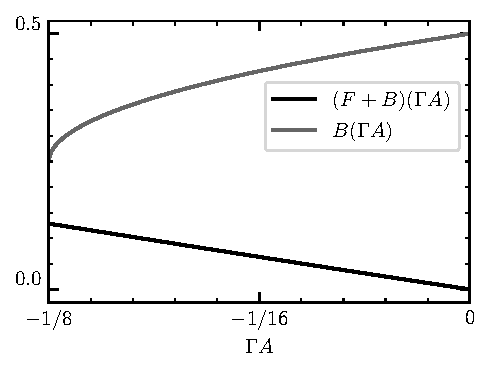
\includegraphics{pictures/k=w_F|B_numn_of_fixp.pdf}
    \vspace*{-2cm}\caption{The cource of $F+B$ and $B$ as function of $\Gamma A$}
    \label{fig:k=w_numb_of_fixp}
\end{wrapfigure}\\
The minimal value of $B$ is taken again in the case $A<0$ for the minus sign and also for $\gamma=0$.\\
For $A<0$ we know that the maximum of $F(y)+B$ is positive, opening the possibility for more than one solution for $y\rightarrow m_y$. In order for this to happen the minimal value of $B$ has to be smaller than the value of the maximum of $F(y)+B$. Both values are determined by $\Gamma A$. Graphically we can see as depicted in \autoref{fig:k=w_numb_of_fixp} that $B$ is always larger than $F(y)$ by noticing, that $F(\Gamma A = 0)=0$, whereas $B(\Gamma A=0)=2$ and $F(\Gamma A = -1/2)\approx0.55$ where $B(\Gamma A= -1/2)=1$.\\
Because $F(y=0)=-B\leq0$ and $F(y\rightarrow-\infty)\rightarrow\infty$, the root of $F(y)$ has to be smaller than $0$ and $0$ for $B=0$.\\\\

Now we take a look at the first eigenvalue of the fixed point.
\begin{align*}
     \lambda_1=-\Gamma\,A-y^2+y
\end{align*}
which has roots at
\begin{align*}
    y_{\pm}=\half\,(1\pm\sqrt{1-4\,\Gamma A})
\end{align*}
\begin{wrapfigure}[13]{l}{0pt}
    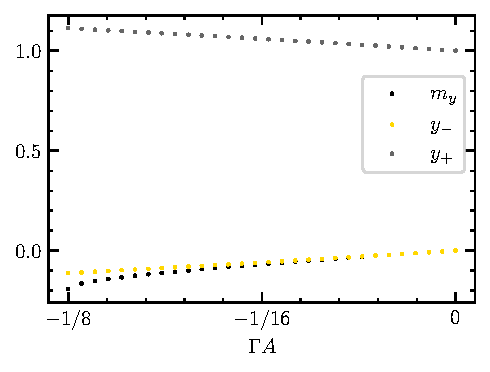
\includegraphics{pictures/k=w_sign_of_ev1.pdf}
    \vspace*{-2cm}\caption{The roots of $\lambda_1$ and the value for $m_y$ for a selection of $\Gamma A$-values.}
    \label{fig:k=w_sign_lam1}
\end{wrapfigure}\\
In order to determine, whether $\lambda_1$ is positive or negative we calculate the roots $m_y$ of $F$ for minimal $B$ in dependence of $\Gamma A$ numerically and compare them to the roots of $\lambda_1$. The minimal $B$ value has been chosen in the above manner as
\begin{align*}
    B=\bigg\{\begin{array}{c l}
          \frac{2\,\Gamma A}{-1-\sqrt{1+8\,\Gamma A}}&\text{for }A<0\\
         0&\text{else}
    \end{array}\quad,
\end{align*}
which corresponds to $\gamma\rightarrow\infty$ for $A>0$.
As seen in the picture $\lambda_1$ is always negative except when $\Gamma A=0$, where it is $0$.\\\\\newpage
Now we can take a look at the other two eigenvalues. For this we analyse the parts of the equation 
\begin{align*}
    0&=t^2+\left( 2\,\frac{\Gamma^2}{\tilde{\kappa}^2}+\Gamma\,A+3\,y^2-4\,y+1  \right)\,t+2\,\frac{\Gamma^2}{\tilde{\kappa}^2}\,\left( \Gamma\,A+3\,y^2-4\,y+1 \right)+2\,\frac{\Gamma^2}{\tilde{\kappa}^2}\,(2\,y-1)\,(y-1)\\
    &=\vcentcolon t^2+p\,t+q
\end{align*}
First $p$ is analysed. It has roots at
\begin{align*}
    t_{\pm}=&\frac{1}{3}\,\left(  2\pm \sqrt{4-3\,(2\Gamma^2/\tilde{\kappa}^2+\Gamma A + 1)} \right)\\
    =&\frac{1}{3}\,\left(  2\pm \sqrt{1-6\,\Gamma^2/\tilde{\kappa}^2-3\,\Gamma A} \right)
\end{align*}
The expression inside the square root is maximized by minimizing $A$ with respect to $\tilde{\kappa}$ and $\gamma$, what results in $\Gamma A = -1/8$, which can be inferred by the previous calculation. As a consequence the expression in the square root is always negative, which means that p is always positive. For the proceeding examination we keep in mind that the eigenvalues are determined by
\begin{align*}
    \lambda_{23}=\half\,(-p\pm\sqrt{p^2-4q})
\end{align*}
If $q$ is positive then both eigenvalues are negative. So let's analyse $q$. 
\begin{align*}
    \frac{q}{2\Gamma^2}=&\Gamma A +1 +\tilde{\kappa}^2-(4+3\,\tilde{\kappa}^2)\,y+(3+2\,\tilde{\kappa}^2)\,y^2\overset{!}{=}0\\
    \Rightarrow\quad y_{12}=&\frac{1}{2\,(3+2\,\tilde{\kappa}^2)}\,\left( 4+3\,\tilde{\kappa}^2\pm \sqrt{16+24\,\tilde{\kappa}^2+9\,\tilde{\kappa}^4-(3+2\,\tilde{\kappa}^2)\,(\Gamma A +1 +\tilde{\kappa}^2)}   \right)\\
    =&\frac{1}{2\,(3+2\,\tilde{\kappa}^2)}\,\left( 4+3\,\tilde{\kappa}^2\pm \sqrt{16+24\,\tilde{\kappa}^2+9\,\tilde{\kappa}^4 -3\,\Gamma A -3 -3\,\tilde{\kappa}^2-2\,(\Gamma A+1)\,\tilde{\kappa}^2-2\,\tilde{\kappa}^4}   \right)\\
    =&\frac{1}{2\,(3+2\,\tilde{\kappa}^2)}\,\left( 4+3\,\tilde{\kappa}^2\pm \sqrt{13-3\,\Gamma A+(19-2\,\Gamma A)\,\tilde{\kappa}^2+7\,\tilde{\kappa}^4}   \right)\\
\end{align*}
Let's look at the term 
\begin{align*}
    3\,\Gamma A +3 +3\,\tilde{\kappa}^2+2\,(\Gamma A+1)\,\tilde{\kappa}^2+2\,\tilde{\kappa}^4
\end{align*}
This term has to become negative in order for one of the $y_{12}$ to get negative too. The $\tilde{\kappa}^2$-roots are found at
\begin{align*}
    \tilde{\kappa}^2_{12}=&\frac{1}{32}\,(-5/2-\Gamma A\pm\sqrt{(5/2+\Gamma A)^2-2\,(3\,\Gamma A+3)})
\end{align*}
Because $3\,\Gamma A+3$ can never become negative in the allowed parameter range, the $\tilde{\kappa}^2$-roots would be negative, which is not possible. Therefore the examined expression can not be negative, which infers that $y_{12}$ is always positive. As we have seen that $m_y$ is always negative, it follows, that $q$ is always positive, which again let's us know, that both eigenvalues $\lambda_{2},\,\lambda_3$ are always negative. which makes the fix point stable and the configuration physically possible.\\\\

In a next step we let be $\tilde{\kappa}\neq\omega$, while $\delta=0$ remains. With the definition $\omega=\tilde{\omega}/\sqrt{2}$ we are looking at the equations
\begin{align*}
    -m_x\,\left(\Gamma A+( m_x^2+ m_y^2)-\frac{\tilde{\omega}}{\tilde{\kappa}}\,m_y\right)  &=0\\\\
    -\frac{\tilde{\omega}\Gamma}{\sqrt{2}\,\tilde{\kappa}^2}-\Gamma A\,m_y    -m_ym_x^2- m_y^3+\frac{\tilde{\omega}}{\tilde{\kappa}}\,(m_x^2+2\,m_y^2)-\frac{\tilde{\omega}^2}{\tilde{\kappa}^2}\,m_y  &=0
\end{align*}
First I show, that also in this case there is no solution for $m_x\neq0$. There we would have
\begin{align*}
    m_x^2=&-m_y^2+\frac{\tilde{\omega}}{\tilde{\kappa}}\,m_y-\Gamma A \\
    \Rightarrow\quad0=&-\frac{\tilde{\omega}\Gamma}{\sqrt{2}\,\tilde{\kappa}^2}-\Gamma A\,m_y    -m_y\,(-m_y^2+\frac{\tilde{\omega}}{\tilde{\kappa}}\,m_y-\Gamma A)- m_y^3+\frac{\tilde{\omega}}{\tilde{\kappa}}\,(-m_y^2+\frac{\tilde{\omega}}{\tilde{\kappa}}\,m_y-\Gamma A+2\,m_y^2)-\frac{\tilde{\omega}^2}{\tilde{\kappa}^2}\,m_y  \\
    =&-\frac{\tilde{\omega}\Gamma}{\sqrt{2}\,\tilde{\kappa}^2}-\frac{\tilde{\omega}}{\tilde{\kappa}}\,\Gamma A\\
    =&-\frac{1}{\sqrt{2}\,\tilde{\kappa}}-\frac{1}{\tilde{\kappa}^2}\,(\Gamma+\gamma-\frac{\tilde{\kappa}}{\sqrt{2}})=-\frac{1}{\tilde{\kappa}^2}\,(\Gamma+\gamma)
\end{align*} 
which is not satisfyable for $\Gamma,\,\gamma\neq0$, which is what we are interested in. So the only possible stationary solutions are
\begin{align*}
    m_x=&0\\
    m_y=&y\\
    \text{with}\quad0=&-\frac{\tilde{\omega}\Gamma}{\sqrt{2}\,\tilde{\kappa}^2}-\Gamma A\,y    - y^3+2\,\frac{\tilde{\omega}}{\tilde{\kappa}}\,y^2-\frac{\tilde{\omega}^2}{\tilde{\kappa}^2}\,y  
\end{align*}
We can multiply the equation with $\tilde{\kappa}^3/\tilde{\omega}^3$, yielding
\begin{align*}
    0=&-\frac{\tilde{\kappa}\Gamma}{\sqrt{2}\,\tilde{\omega}^2}-(\frac{\tilde{\kappa}^2}{\tilde{\omega}^2}\,\Gamma A+1)\,\frac{\tilde{\kappa}}{\tilde{\omega}}\,y    - \frac{\tilde{\kappa}^3}{\tilde{\omega}^3}\,y^3+2\,\frac{\tilde{\kappa}^2}{\tilde{\omega}^2}\,y^2 
\end{align*}
when we now redefine $\tilde{y}\vcentcolon=y\tilde{\kappa}/\tilde{\omega}$ and $\Gamma\tilde{A}\vcentcolon=\tilde{\kappa}^2/\tilde{\omega}^2\,\Gamma A$ we can restate the solution as
\begin{align*}
    m_x=&0\\
    m_y=&\tilde{\omega}/\tilde{\kappa}\,\tilde{y}\\
    \text{with}\quad0=&-\frac{\tilde{\kappa}^2}{\tilde{\omega}^2}\,B-(\Gamma \tilde{A}+1)\,\tilde{y}    - \tilde{y}^3+2\,\tilde{y}^2=\vcentcolon F'(\tilde{y})
\end{align*}
with the previous defined $B$. $\Gamma \tilde{A}$ can now take all real numbers as values. The analysis concerning the number of existent $m_y$-solutions is the same with a prefactor in front of $B$. 
\begin{align*}
    B'\vcentcolon=&\frac{\tilde{\kappa}^2}{\tilde{\omega}^2}\,B=\frac{2\,\Gamma \tilde{A}}{-1\pm\sqrt{1+8A\,(\Gamma+\gamma)}}
\end{align*}
$B'$ can be rewritten, so that the question of the number of fixed points can be discussed with only two parameters
\begin{wrapfigure}[14]{l}{0pt}
    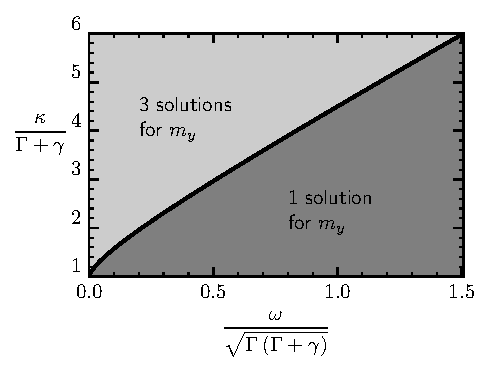
\includegraphics{pictures/numb_fixp.pdf}
    \vspace*{-2cm}\caption{The number of fixed points depending on the parameter configuration.}
    \label{fig:numb_fixp}
\end{wrapfigure}\\ 
% \begin{figure}[H]
%     \floatbox[{\capbeside\captionsetup[capbesidefigure]{labelsep=newline}%
%     \thisfloatsetup{capbesideposition={right,center},capbesidewidth=none}}]{figure}[\FBwidth]
%     {\caption{The course of $F'+B'$ and $B'$ as function of $\Gamma\tilde{y}$.\\\\As the value of the maximum of $F'$ with $B'=0$ grows faster than linear, there are parameter configurations with three different fixed points. As the $B'$ can also grow infinitly for a given value of $\Gamma\tilde{A}$. There are also parameter regimes possible with only one fixed point.}}
%     {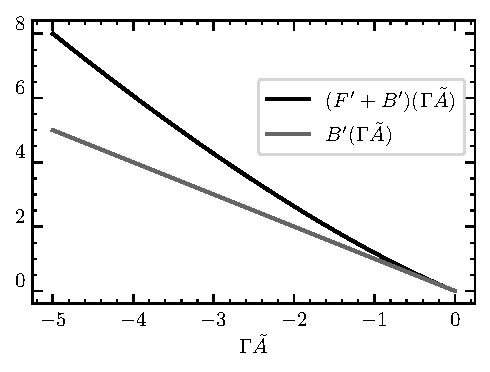
\includegraphics{pictures/numn_of_fixp.pdf}}
%     %{\label{fig:num_of_fixp_criterium_BF}}
% \end{figure}
\begin{align*}
    B'=&\frac{1}{\tw^2}\,\frac{2\,\Gamma\,(\Gamma+\gamma)\,(1-\frac{\tk}{\sqrt{2}})}{-1\pm\sqrt{1+8\,\frac{(\Gamma+\gamma)^2}{\tk^2}\,(1-\frac{\tk}{\sqrt{2}})}}
\end{align*}
With the rescaling $\Omega=\tw/\sqrt{2\,\Gamma\,(\Gamma+\gamma)}$ and $K=\tk/(\sqrt{2}\,(\Gamma+\gamma))$ we get
\begin{align*}
    B'=&\frac{K}{2\,\Omega^2}\\
    \text{and}\quad y_\text{max}=&\frac{1}{3}\,\left( 2+ \sqrt{1-\frac{3}{2}\,(1-K)\,\frac{1}{\Omega^2}}  \right)
\end{align*}
In this way we can compute the border between the configurations with different numbers of fixed points numerically. As we know from previous considerations if $\tilde{A}>0$ which corresponds to $K>1$ the maximum of $F'$ is negative even for $B'=0$
% \begin{figure}[H]
%     \hspace*{-1cm}
%     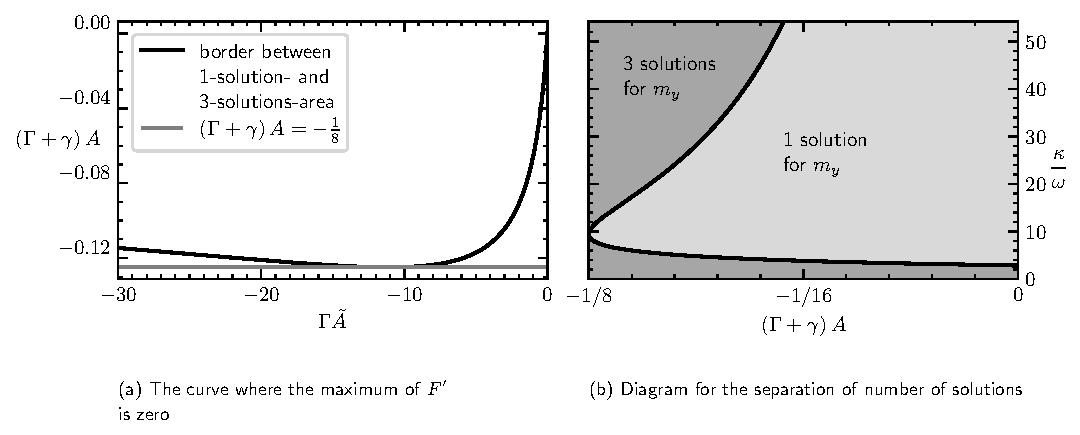
\includegraphics{pictures/phaseplot_A_kw.pdf}
%     \caption{The parameter configurations, where there are 1 ore 3 fixed points can be separated.}
%     \label{fig:phases_numb_of_fixp}
% \end{figure}
We proceed again by calculating the linear expansion of the differential equations.
\begin{align*}
    \dt\left(\begin{array}{c}
         \delta m_x\\
         \delta m_y\\
         \delta m_z
    \end{array}\right)=&\left( \begin{array}{ccc}
        -\Gamma\,A-y^2+\frac{\tilde{\omega}}{\tilde{\kappa}}\,y&  0 & 0\\
        0 & -\Gamma\,A-3\,y^2+4\,\frac{\tilde{\omega}}{\tilde{\kappa}}\,y-\frac{\tilde{\omega}^2}{\tilde{\kappa}^2} & \sqrt{2}\,\frac{\Gamma^2}{\tilde{\kappa}^2}\,(\tilde{\kappa}\,y-\tilde{\omega})\\
        0 &  -\sqrt{2}\,\frac{\Gamma}{\tilde{\kappa}^2}\,(2\tilde{\kappa}\,y-\tilde{\omega}) & -2\,\frac{\Gamma^2}{\tilde{\kappa}^2}
    \end{array} \right)\,\left(\begin{array}{c}
         \delta m_x\\
         \delta m_y\\
         \delta m_z
    \end{array}\right)
\end{align*}
For the analysis of the sign of the eigenvalues we are free to multiply the matrix with a positiv number, i.e $\tilde{\kappa}^2/\tilde{\omega}^2$, what yields the matrix
\begin{align*}
    \mathcal{A}=\left( \begin{array}{ccc}
        -\Gamma\tilde{A}-\tilde{y}^2+\tilde{y}&  0 & 0\\
        0 & -\Gamma\tilde{A}-3\,\tilde{y}^2+4\,\tilde{y}-1 & \sqrt{2}\,\Gamma/\tilde{\kappa}\,(\tilde{y}-\frac{\tilde{\kappa}}{\tilde{\omega}})\\
        0 &  -\sqrt{2}\,\Gamma/\tilde{\kappa}\,(2\,\tilde{y}-\frac{\tilde{\kappa}}{\tilde{\omega}}) & -2\,\frac{\Gamma^2}{\tilde{\omega}^2}
    \end{array} \right)
\end{align*}
The first eigenvalue has the same form as previously. Here we have to analyse it's sign for all 3 possible fixed points.\newpage
\begin{wrapfigure}[16]{l}{0pt}
    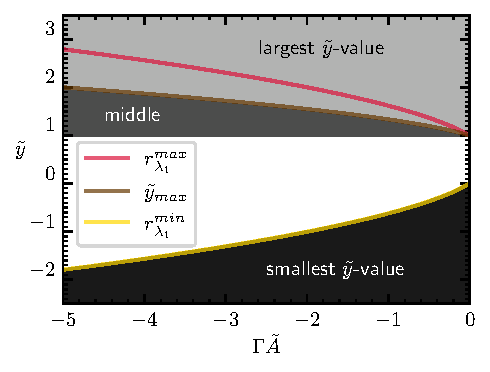
\includegraphics{pictures/sign_of_ev1.pdf}
    \vspace*{-2cm}\caption{The smaller ($r_{\lambda_1}^{min}$) and larger ($r_{\lambda_1}^{max}$) roots of $\lambda_1$ with marked areas for the value for $\tilde{y}=k/w\cdot m_y$. $\tilde{y}_{max}$ is the $\tilde{y}$-position of $F'$.}
    \label{fig:sign_lam1}
\end{wrapfigure}
In order to allow ourselves to answer the question about the sign of the first eigenvalue in general, we again define an even more general parameter
\begin{align*}
    \chi\vcentcolon=&\frac{K-1}{\Omega^2}\\
    \Rightarrow\quad\Gamma\tilde{A}=&-\half\,\chi\\
    \frac{K}{2\,\Omega^2}=&\frac{K-1}{2\,\Omega^2}+\frac{1}{2\,\Omega^2}=\half\,\chi+\frac{1}{2\,\Omega^2}
\end{align*}
For a given value of $\chi$ the parameter $\Omega$ can be choosen freely, because through an appropriate choice of $K$ the value of $\chi$ can be fixed. So for every possible value of $chi>0$ the supremal value of $B'$ is just $\chi/2$, as $\Omega\rightarrow\infty$.
The first, smallest fixed point has again because of the positive sign of $B'$ always a negative $y$-components. It has it's greatest value for minimal $B'$. Negative values of $\chi$ lead to positive roots of $\lambda_1$, which induces that $\lambda_1$ itself is negative. \\\\
So we only have to consider positive $\chi$-values, in rememberence of fact, that there is only one fixed point for $\chi<0$ . It turns out that the smaller root of $\lambda_1$ is always a root of $F'$ (for $B'=\chi/2$) which always represents $F'$'s smallest root, which can be checked by calculating the slope of $F'$ at this point.
\begin{align*}
    F'(\tilde{y})=-\half\,\chi-(1-\half\,\chi)\,\tilde{y}    - \tilde{y}^3+2\,\tilde{y}^2
\end{align*}
So we can move on to the next fixed point, the one in the middle. It takes it's smallest value for minimal $B'$. In this constellation the middle root turns out to be always at $\tilde{y}=1$. The maximal possible value (actually supremum) for the middle root is at the maximum point of $F'$ which is also the minimal possible value of the largest root. So we can already provide a diagramm for the possible sign-values of $\lambda_1$ in \autoref{fig:sign_lam1}.\\\\
At this point I want to discuss which of the above computed fixed points are physical ones, meaning $|m|<=1/2$. Therefore we consider the total mean angular momentum.
\begin{align*}
    m_z=&\half-\frac{1}{\Gamma}\,\left( \kappa\,(m_x^2+m_y^2)-\omega m_y  \right)\\
    =&\half-\frac{\kappa}{\Gamma}\,\left( m_y^2-\frac{\omega}{\kappa}\, m_y  \right)\\
    \Rightarrow\quad |m|^2=&\left( \half-\frac{\kappa}{\Gamma}\,\left( m_y^2-\frac{\omega}{\kappa}\, m_y  \right) \right)^2+m_y^2\\
    =&\left( \half-\frac{\omega^2}{\Gamma\kappa}\,\left( \tilde{y}^2- \tilde{y} \right) \right)^2+\frac{\omega^2}{\kappa^2}\,\tilde{y}^2\\
    =&\left( \half-\frac{\Omega^2}{K}\,\left( \tilde{y}^2- \tilde{y} \right) \right)^2+\frac{\Gamma}{\Gamma+\gamma}\,\frac{\Omega^2}{K^2}\,\tilde{y}^2\\
    \leq&\left( \half-\frac{\Omega^2}{K}\,\left( \tilde{y}^2- \tilde{y} \right) \right)^2+\frac{\Omega^2}{K^2}\,\tilde{y}^2\\
    =&\vcentcolon m^*
\end{align*}

Now I set $\Omega^2/K$ through the determining equation for $m_y$.
\begin{align*}
    0=&-\frac{K}{2\Omega^2}-\left( \frac{1-K}{2\Omega^2} +1\right)\,\tilde{y}-\tilde{y}^2+2\,\tilde{y}^2\\
    \Rightarrow\quad \frac{K}{2\Omega^2}\,(\tilde{y}-1)=&(1+\frac{1}{2\Omega^2})\,\tilde{y}+\tilde{y}^3-2\,\tilde{y}^2\\
    \frac{\Omega^2}{K}=&\frac{\tilde{y}-1}{2\,\left(  (1+\frac{1}{2\Omega^2})\,\tilde{y}+\tilde{y}^3-2\,\tilde{y}^2\right)}
\end{align*}
\begin{align*}
    \frac{\text{d}}{\text{d}\tilde{y}}\,\frac{\Omega^2}{K}=&\frac{1}{2\,\left(  (1+\frac{1}{2\Omega^2})\,\tilde{y}+\tilde{y}^3-2\,\tilde{y}^2\right)}-\frac{2\,(\tilde{y}-1)\,(1+\frac{1}{2\Omega^2}+3\,\tilde{y}^2-4\,\tilde{y})}{4\,\left(  (1+\frac{1}{2\Omega^2})\,\tilde{y}+\tilde{y}^3-2\,\tilde{y}^2\right)^2}\\\\
    =&\frac{1+\frac{1}{2\Omega^2}-4\,\tilde{y}+5\,\tilde{y}^2-2\,\tilde{y}^3}{2\,\left(  (1+\frac{1}{2\Omega^2})\,\tilde{y}+\tilde{y}^3-2\,\tilde{y}^2\right)^2}
\end{align*}

This equation looks at first strange, because $k/2\Omega^2$ could be negative for $0<\tilde{y}<1$. But as we've already seen in \autoref{fig:sign_lam1}, this space is free of fixed points. \\\\
Taking the derivative of $m^*$
\begin{align*}
    \frac{\partial m^*}{\partial\tilde{y}}=&-2\,\left(\frac{\Omega^2}{K}\,(2\tilde{y}-1)+\left(\frac{\text{d}}{\text{d}\tilde{y}}\,\frac{\Omega^2}{K}\right)\,(\tilde{y}^2-\tilde{y})\right)\,\left( \half-\frac{\Omega^2}{K}\,\left( \tilde{y}^2- \tilde{y} \right) \right)+2\,\frac{\Omega^2}{K^2}\,\tilde{y}+2\,\left(\frac{\text{d}}{\text{d}\tilde{y}}\,\frac{\Omega^2}{K}\right)\,\frac{\Omega^2}{K}\,\frac{1}{\Omega^2}\,\tilde{y}^2\\
    % =&4\,(\frac{\Omega^2}{K})^2\,\tilde{y}^3-\left(2\,(\frac{\Omega^2}{K})^2+4\,(\frac{\Omega^2}{K})^2\right)\,\tilde{y}^2+\left( 2\,(\frac{\Omega^2}{K})^2+2\,\frac{\Omega^2}{K^2}-2\,\frac{\Omega^2}{K} \right)\,\tilde{y}+\frac{\Omega^2}{K}\\
    % =&\frac{\Omega^2}{K}\,\left[  4\,\frac{\Omega^2}{K}\,\tilde{y}^3-6\,\frac{\Omega^2}{K}\,\tilde{y}^2+\left( 2\,\frac{\Omega^2}{K}+2\,\frac{\Omega^2}{K}\,\frac{1}{\Omega^2}-2 \right)\,\tilde{y}+1 \right]
\end{align*}

So plugging the found result into the equation for the derivative of $m^*$ yields
\begin{align*}
    \frac{2\,\left[(1+\frac{1}{2\Omega^2})\,\tilde{y}+\tilde{y}^3-2\,\tilde{y}^2\right]^2}{\tilde{y}-1}\,\frac{\partial m^*}{\partial\tilde{y}}=&2\,(\tilde{y}-1)\,\tilde{y}^3-3\,(\tilde{y}-1)\,\tilde{y}^2\\
    &+\left( \tilde{y}-1+(\tilde{y}-1)\,\frac{1}{\Omega^2}-2\,\left((1+\frac{1}{2\Omega^2})\,\tilde{y}+\tilde{y}^3-2\,\tilde{y}^2\right) \right)\,\tilde{y}\\
    &+(1+\frac{1}{2\Omega^2})\,\tilde{y}+\tilde{y}^3-2\,\tilde{y}^2 \\\\
    =&3\,\tilde{y}^2+\left( -(1+\frac{1}{\Omega^2})-\tilde{y}\right)\,\tilde{y}+(1+\frac{1}{2\Omega^2})\,\tilde{y}-2\,\tilde{y}^2\\
    =&-\frac{1}{2\Omega^2}\,\tilde{y}\\\\
    \Rightarrow\quad\frac{\partial m^*}{\partial\tilde{y}}=&-\frac{\tilde{y}-1}{2\,\left[(1+\frac{1}{2\Omega^2})\,\tilde{y}+\tilde{y}^3-2\,\tilde{y}^2\right]^2}\,\frac{1}{2\Omega^2}\,\tilde{y}
\end{align*}



% \\\\

The other two eigenvalues are defined through the solution of the following equation
\begin{align*}
    0&=t^2+\left( 2\,\frac{\Gamma^2}{\tilde{\omega}^2}+\Gamma\,\tilde{A}+3\,\tilde{y}^2-4\,\tilde{y}+1  \right)\,t+2\,\frac{\Gamma^2}{\tilde{\omega}^2}\,\left( \Gamma\,\tilde{A}+3\,\tilde{y}^2-4\,\tilde{y}+1 \right)+2\,\frac{\Gamma^2}{\tilde{\kappa}^2}\,(2\,\tilde{y}-\frac{\tilde{\kappa}}{\tilde{\omega}})\,(\tilde{y}-\frac{\tilde{\kappa}}{\tilde{\omega}})\\
    &=\vcentcolon t^2+p\,t+q
\end{align*}
Starting with the analysis of $p$ and rewriting with the new parameters, we find 
\begin{align*}
    p=&\frac{\Gamma}{\Omega^2\,(\Gamma+\gamma)}-\half\,\chi+3\,\tilde{y}^2-4\,\tilde{y}+1
\end{align*}
the roots of this expression, which are maximally apart from each other, are found, when $\Omega\rightarrow\infty$ in the same spirit as above. This yields as roots of $p$
\begin{align*}
    r_p=&\frac{1}{3}\,\left( 2\pm\sqrt{1+\frac{3}{2}\,\chi-3\,\frac{\Gamma}{\Omega^2\,(\Gamma+\gamma)}} \right)\\
    \Rightarrow\quad r_p^\text{max}=&\frac{1}{3}\,\left( 2+\sqrt{1+\frac{3}{2}\,\chi} \right)\\
    r_p^\text{min}=&\frac{1}{3}\,\left( 2-\sqrt{1+\frac{3}{2}\,\chi} \right)
\end{align*}
We can recognize, that $r_p^\text{max}=\tilde{u}_\text{max}$ and $r_p^\text{min}=\tilde{u}_\text{min}$. Thus we can infer that for the bracketing fixed points $p$ is always positive, whereas for the middle fixed point we can't make this statement.

\begin{figure*}
    \centering
    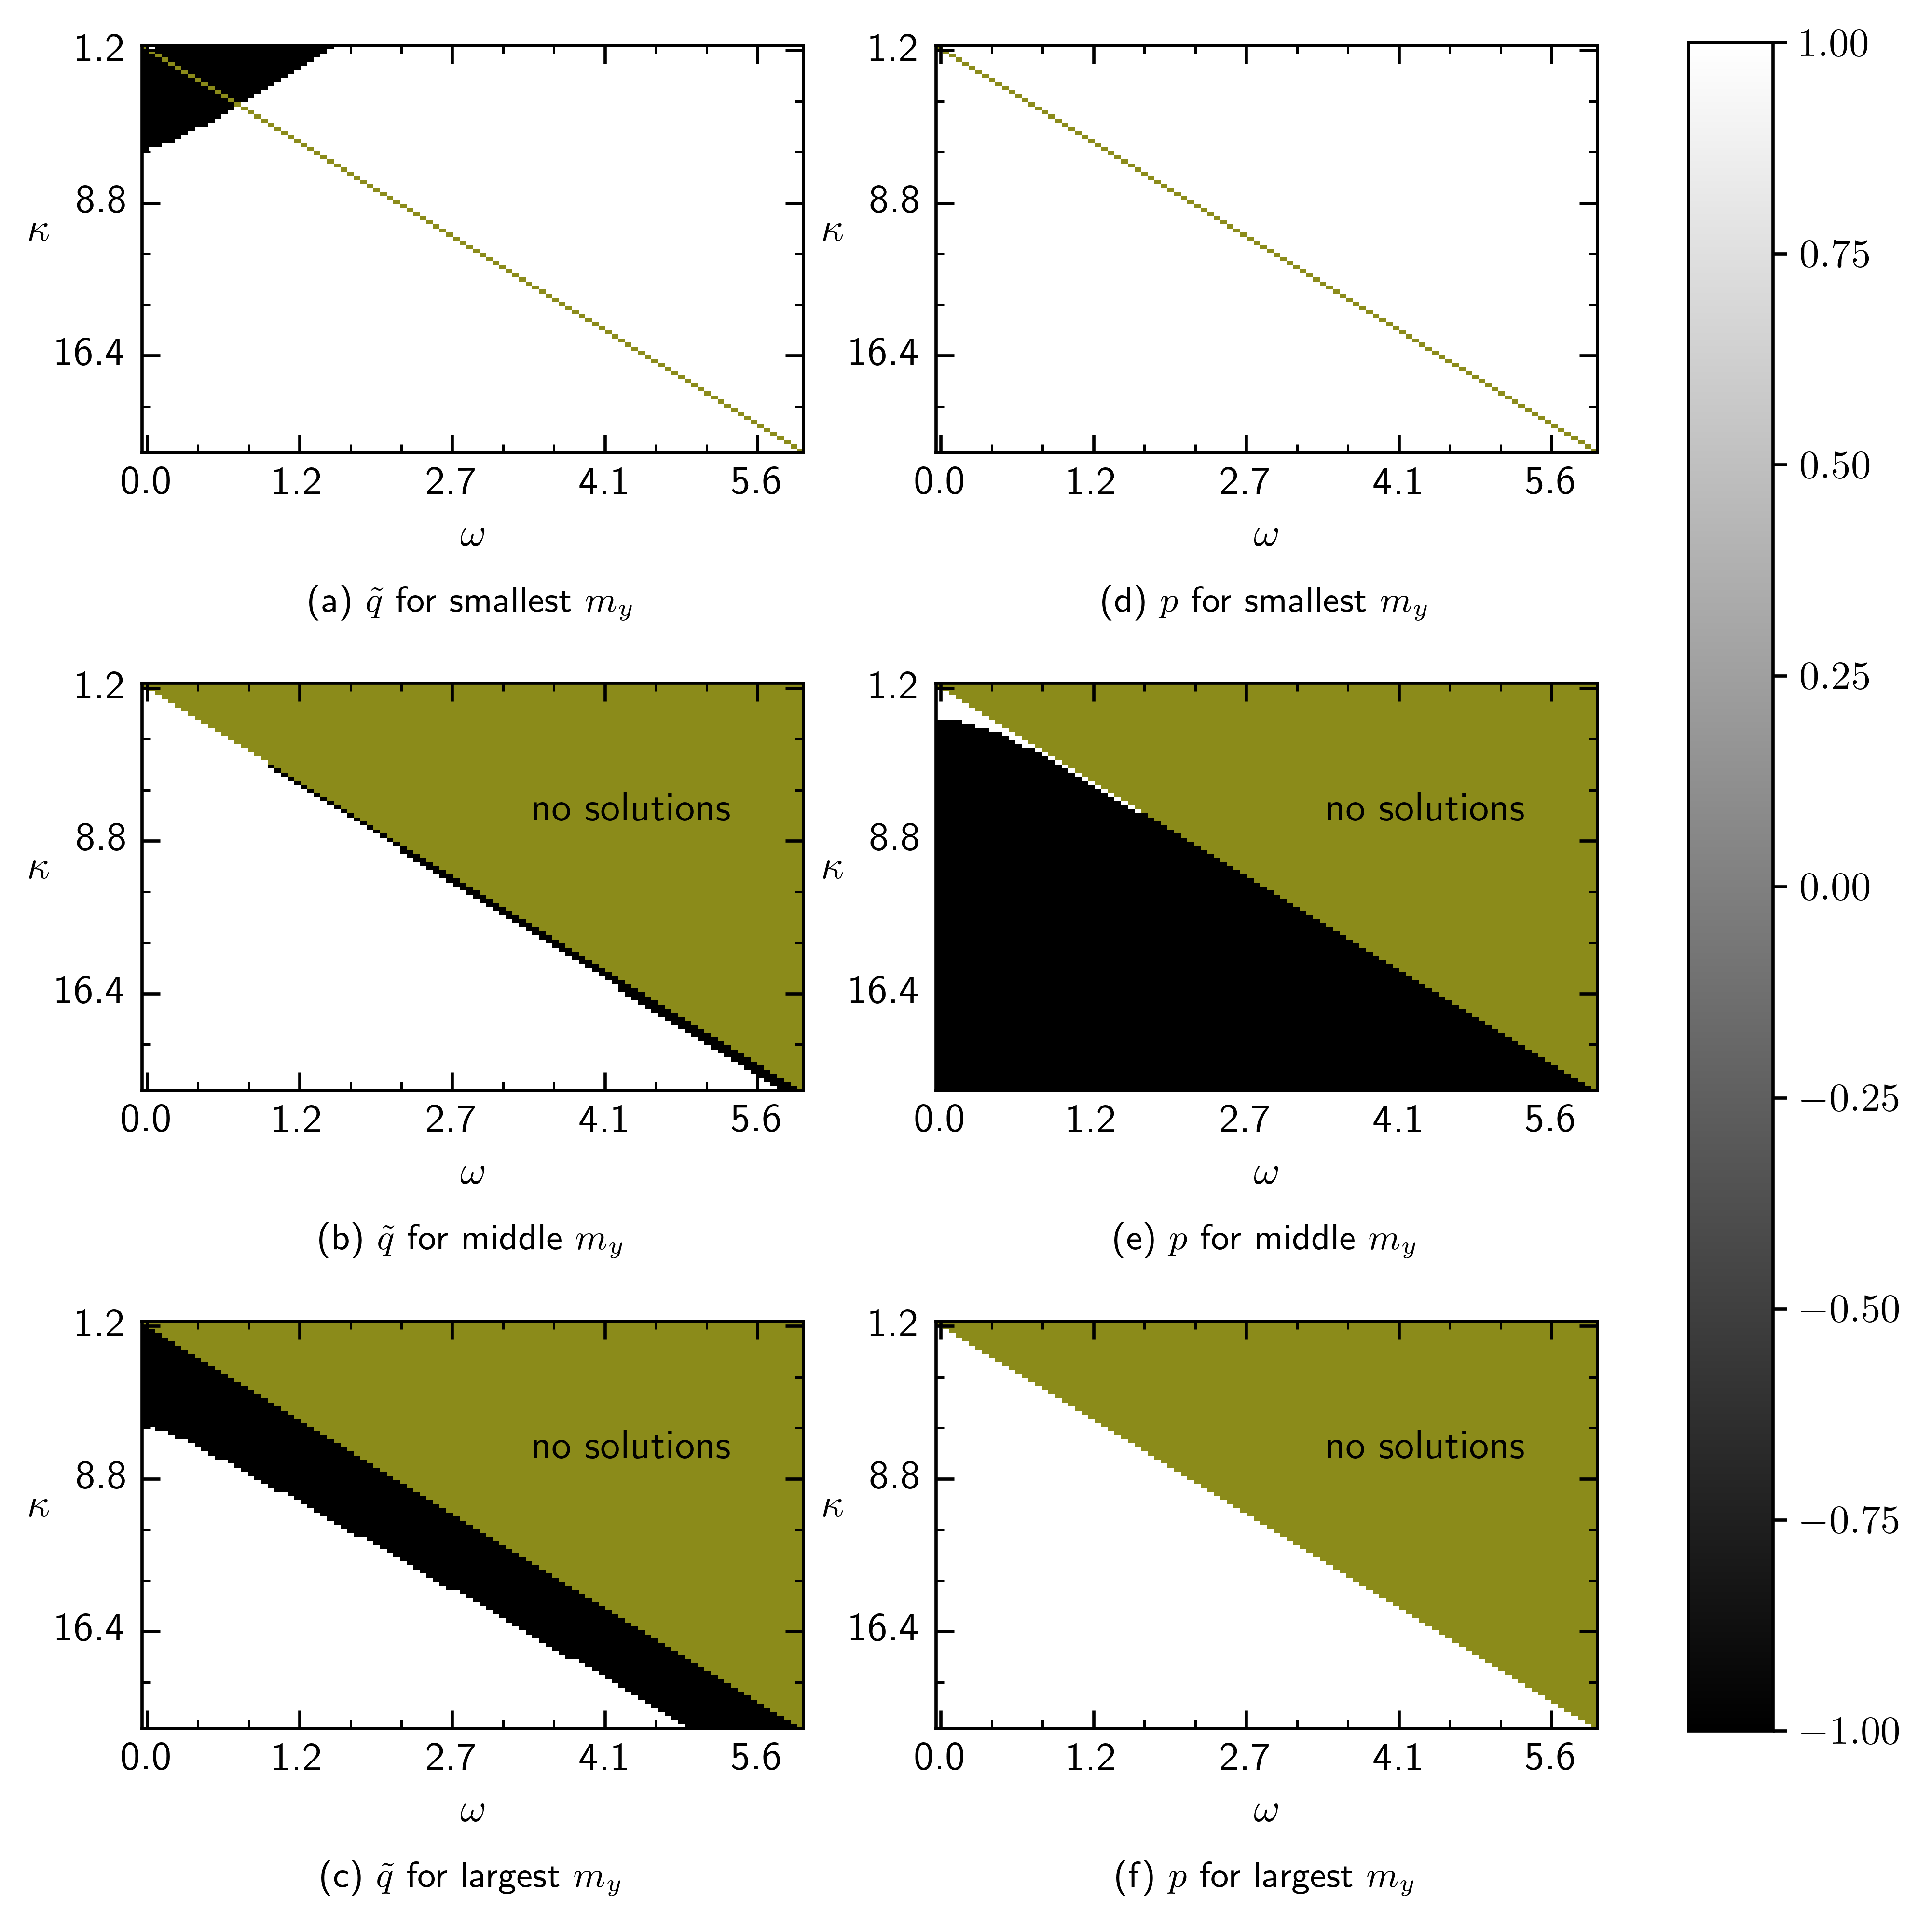
\includegraphics{pictures/lam2_anal.png}
    \caption{The yellow line signals in each plot the border between the area with one vs. more than one fix points. Above the line there is only one fixed point. The figures a-c present the sign of the interior of the square root for the eigenvalues $\lambda_{23}$ for different parameter configurations-in the lower segment of the plots for the fixed point specified int the subcaption, in the upper segment for the only fixed point, which is why the plots look the same in this part. Figures d-f show in the same manner the sign of $p$. In the entire setup is $\Gamma=1$ and $\gamma=0.2$ fixed.}
\end{figure*}




\newpage
\appendix
\section*{Appendix}

\subsection*{The J-square calculus}
If there is a system of $N$ coupled ODE, this could be seen as the quest for a function $\vec{F}:\,\mathbb{R}\rightarrow\mathbb{R}^N$. Derived from that, there can also be defined the function squared $F^2:\,\mathbb{R}\rightarrow\mathbb{R}:\,t\mapsto\sum_{i=1}^NF_i^2(t)$. If one is now able to write the derivative of squared function in the following way
\begin{align*}
    \dt F^2(t)=&\vec{F}^t(t)\,A\,\vec{F}(t)
\end{align*}
with a Matrix $A$, which is positive ore negative definite, then there do not exist stationary solutions to the system of ODE, including limit cycles. \\
\textit{Proof}: The functions $\vec{F}$, can be mapped via N-dimensional spherical coordinates into a different set of functions $f(t)$, $\varphi_j(t)$ $j\in\{1,\dots,N-1\}$, with $f$ the modulus of $F$, and $\varphi_j$ the angles. This is true for all solutions $\vec{F}\neq\vec{0}$. In the following we neglect this special case, as this is in the most cases anyway a stationary point. With the notation.
\begin{align*}
    \vec{F}(t)=&f(t)\,\hat{r}(t)
\end{align*}
we can rewrite the differential equation for the squared function to
\begin{align*}
    \dt F^2(t)=\dt f^2(t)=2\,f(t)\,\dt f(t)=&f^2(t)\,\hat{r}^t\,A\,\hat{r}\\
    \Rightarrow\quad\dt f(t) = f(t)\,\hat{r}^t\,A\,\hat{r}
\end{align*}
Assuming that A is positive or negative definite we can use the property that $|\hat{r}(t)|=1\,\forall t$, in order to follow, that there exists an $\varepsilon>0$ so that
\begin{align*}
    \lambda(t)\vcentcolon=\left| \hat{r}^t(t)\,A\,\hat{r}(t) \right| > \varepsilon
\end{align*}
For all $t$ and all functions $\{\varphi_j(t)\}$. \textit{Proof}: if this doesn't hold, there will have to be a sequence $(t_n)$ with $\lambda(t_n)\rightarrow0$. As the surface of an N-dimensional sphere is a compact set, this sequence would have to converge on the survace of the sphere, which would infer $\exists \hat{r}\neq0$ with 
\begin{align*}
    \hat{r}^t(t)\,A\,\hat{r}(t)=0
\end{align*}
in contradiction to the definiteness of $A$. So depending on, whether $A$ is positive or negative definite, we can write
\begin{align*}
    \dt f(t) >& \varepsilon\,f(t)\\
    \Rightarrow\quad f(t) >& c\,e^{\varepsilon\,t}\\
    \text{or}\quad \dt f(t) <& -\varepsilon\,f(t)\\
    \Rightarrow\quad f(t) <& c\,e^{-\varepsilon\,t}\\
\end{align*}
for suitable choice of $c$ (can be shown with mean value theorem). This implies, that there can't be a stationary solution of the set of ODE. The last statement holds, because for $t\rightarrow\infty$ either $f$ goes to zero, which would imply that all $F_i$ go to zero or $f$ grows boundlessly, which implies that, independent of the starting conditions, there exists a $F_i$, that grows boundlessly, which forbids the properties of a stationary state including limit cycles.





\subsection*{Very general ancilla state}
The following attempt tries to get better mean field in a different global system by changing the states, the ancillas occupy. Therefore we choose a mixed state of generall quantum states.
\begin{align*}
    \eta =& p \, \ket{\psi_1}\bra{\psi_1}+ q \, \ket{\psi_2}\bra{\psi_2}\\
    \text{where}\quad p+q=&1\\
    \text{and}\quad \ket{\psi_{1}}=&\frac{1}{\sqrt{2}}\,\left(d\ket{\uparrow} + c\ket{\downarrow}\right)\\
    \ket{\psi_{2}}=&\frac{1}{\sqrt{2}}\,\left(c\ket{\uparrow} \pm d\ket{\downarrow}\right)
\end{align*}

So
\begin{align*}
      \Braket{\psi_{1}| V_n| \psi_{1}}=&\half\left(d^*\bra{\uparrow}+ c^*\bra{\downarrow}\right) \,\tilde{g}\,\left[\alpha_x\,J_x\,\sigma_x+\alpha_y\,J_y\,\sigma_y+\alpha_z\,J_z\,\sigma_z\right] \,\left(d\ket{\uparrow}+ c\ket{\downarrow}\right)\\
    =&\half\left(d^*\bra{\uparrow}+c^*\bra{\downarrow}\right) \,\tilde{g}\,\left[\alpha_x\,J_x\,\left(d\ket{\downarrow}+c\ket{\uparrow}\right)+i\,\alpha_y\,J_y\,\left(d\ket{\downarrow}-c\ket{\uparrow}\right)+\alpha_z\,J_z\,\left(d\ket{\uparrow}-c\ket{\downarrow}\right)\right]\\
    =&\half\tilde{g}\,\left[\alpha_xJ_x\,(+ d^*c+ c^*d ) + i\,\alpha_yJ_y\,(- d^*c+ c^*d) + \alpha_zJ_z\,(|d|^2-|c|^2)\right]\\
    =&\tilde{g}\,\left[\alpha_xJ_x\,\mathfrak{Re} [d^*c] + \alpha_yJ_y\,\mathfrak{Im} [d^*c] + \alpha_zJ_z\,\half\,(|d|^2-|c|^2)\right]\\
%
 %   
    \Braket{\psi_{2}| V_n| \psi_{2}}=&\half\left(c^*\bra{\uparrow}\pm d^*\bra{\downarrow}\right) \,\tilde{g}\,\left[\alpha_x\,J_x\,\sigma_x+\alpha_y\,J_y\,\sigma_y+\alpha_z\,J_z\,\sigma_z\right] \,\left(c\ket{\uparrow}\pm d\ket{\downarrow}\right)\\
    =&\half\left(c^*\bra{\uparrow}\pm d^*\bra{\downarrow}\right) \,\tilde{g}\,\left[\alpha_x\,J_x\,\left(c\ket{\downarrow}\pm d\ket{\uparrow}\right)+i\,\alpha_y\,J_y\,\left(c\ket{\downarrow}\mp d\ket{\uparrow}\right)+\alpha_z\,J_z\,\left(c\ket{\uparrow}\mp d\ket{\downarrow}\right)\right]\\
    =&\half\tilde{g}\,\left[\alpha_xJ_x\,(\pm c^*d\pm d^*c ) + i\,\alpha_yJ_y\,(\mp c^*d\pm d^*c) + \alpha_zJ_z\,(|c|^2-|d|^2)\right]\\
    =&\tilde{g}\,\left[\pm\alpha_xJ_x\,\mathfrak{Re} [c^*d] \pm \alpha_yJ_y\,\mathfrak{Im} [c^*d] + \alpha_zJ_z\,\half\,(|c|^2-|d|^2)\right]\quad,
\end{align*}
where we used $|c|^2+|d|^2=2$. For a simpler notation it is defined $\mathfrak{Re} [c^*d]=\vcentcolon\lambda$, $\mathfrak{Im} [c^*d]=\vcentcolon\mu$, $|d|^2-|c|^2=\vcentcolon2\gamma$.
\begin{align*}
    \Braket{\psi_{1}| V_n| \psi_{2}}=&\half\left(d^*\bra{\uparrow}+ c^*\bra{\downarrow}\right) \,\tilde{g}\,\left[\alpha_x\,J_x\,\sigma_x+\alpha_y\,J_y\,\sigma_y+\alpha_z\,J_z\,\sigma_z\right] \,\left(c\ket{\uparrow}\pm d\ket{\downarrow}\right)\\
    =&\half\left(d^*\bra{\uparrow}+ c^*\bra{\downarrow}\right) \,\tilde{g}\,\left[\alpha_x\,J_x\,\left(c\ket{\downarrow}\pm d\ket{\uparrow}\right)+i\,\alpha_y\,J_y\,\left(c\ket{\downarrow}\mp d\ket{\uparrow}\right)+\alpha_z\,J_z\,\left(c\ket{\uparrow}\mp d\ket{\downarrow}\right)\right]\\
    =&\half\tilde{g}\,\left[\alpha_xJ_x\,(|c|^2\pm |d|^2 ) + i\,\alpha_yJ_y\,(|c|^2\mp |d|^2 ) + \alpha_zJ_z\,(d^*c\mp c^*d)\right]\\
    =&\tilde{g}\,\left[\alpha_xJ_x+ i\,\alpha_yJ_y\,\half\,(|c|^2 - |d|^2 ) -i\, \alpha_zJ_z\,\mathfrak{Im}[c^*d]\right]\quad\text{for }+\\
    =&\tilde{g}\,\left[\alpha_xJ_x\,\half\,(|c|^2 - |d|^2 )+ i\,\alpha_yJ_y\, +\, \alpha_zJ_z\,\mathfrak{Re}[c^*d]\right]\quad\text{for }-.
\end{align*}
From this the Lindblad operators can be inferred,\\
For $+$
\begin{align*}
    L_{11}=&g\sqrt{p}\,\left[\lambda \alpha_xJ_x +\mu\alpha_yJ_y +\gamma\alpha_zJ_z\right]\\
    L_{22}=&g\sqrt{q}\,\left[\lambda \alpha_xJ_x +\mu\alpha_yJ_y -\gamma\alpha_zJ_z\right]\\
    L_{12}=&g\sqrt{p}\,\left[\alpha_xJ_x +i\,\gamma\alpha_yJ_y +i\,\mu \alpha_zJ_z\right]\\
    L_{21}=&g\sqrt{q}\,\left[\alpha_xJ_x -i\,\gamma\alpha_yJ_y -i\,\mu \alpha_zJ_z\right]
\end{align*}
And for $-$
\begin{align*}
    L_{11}=&g\sqrt{p}\,\left[\lambda \alpha_xJ_x +\mu\alpha_yJ_y +\gamma\alpha_zJ_z\right]\\
    L_{22}=&g\sqrt{q}\,\left[-\lambda \alpha_xJ_x -\mu\alpha_yJ_y -\gamma\alpha_zJ_z\right]\\
    L_{12}=&g\sqrt{p}\,\left[-\gamma\alpha_xJ_x -i\,\alpha_yJ_y +\lambda \alpha_zJ_z\right]\\
    L_{21}=&g\sqrt{q}\,\left[-\gamma\alpha_xJ_x +i\,\alpha_yJ_y +\lambda \alpha_zJ_z\right]
\end{align*}
In the following we will focus on the equations for the case of a plus sign in the definition of $\ket{\psi_2}$. Calculating again the terms involved in the ME, one finds
\begin{align*}
    L_{11}L_{11}^\dagger=&g^2\,p\,\big(\lambda^2\alpha_x^2J_x^2+\mu^2\,\alpha_y^2J_y^2+\gamma^2\alpha_z^2J_z^2\\
    &+\lambda\gamma\alpha_x\alpha_z\,(J_xJ_z+J_zJ_x)+\mu\gamma\alpha_y\alpha_z\,(J_yJ_z+J_zJ_y)+\lambda\mu\alpha_x\alpha_y\,(J_xJ_y+J_yJ_x)\big)\\
    L_{22}L_{22}^\dagger=&g^2\,q\,\big(\lambda^2\alpha_x^2J_x^2+\mu^2\,\alpha_y^2J_y^2+\gamma^2\alpha_z^2J_z^2\\
    &-\lambda\gamma\alpha_x\alpha_z\,(J_xJ_z+J_zJ_x)-\mu\gamma\alpha_y\alpha_z\,(J_yJ_z+J_zJ_y)+\lambda\mu\alpha_x\alpha_y\,(J_xJ_y+J_yJ_x)\big)\\
    L_{12}L_{12}^\dagger=&g^2\,p\,\big(\gamma^2\alpha_x^2J_x^2+\alpha_y^2J_y^2+\mu^2\alpha_z^2J_z^2\\
    &-i\,\mu\alpha_x\alpha_z\,(J_xJ_z-J_zJ_x)+\gamma\mu\alpha_y\alpha_z\,(J_yJ_z+J_zJ_y)-i\,\gamma\alpha_x\alpha_y\,(J_xJ_y-J_yJ_x)\big)\\
    L_{21}L_{21}^\dagger=&g^2\,q\,\big(\gamma^2\alpha_x^2J_x^2+\alpha_y^2J_y^2+\mu^2\alpha_z^2J_z^2\\
    &+i\,\mu\alpha_x\alpha_z\,(J_xJ_z-J_zJ_x)+\gamma\mu\alpha_y\alpha_z\,(J_yJ_z+J_zJ_y)+i\,\gamma\alpha_x\alpha_y\,(J_xJ_y-J_yJ_x)\big)
\end{align*}
Plugging these results in into the terms of the ME yields.
\begin{align*}
    \sum_{kk'}L_{kk'}\rho\L_{kk'}^\dagger=&g^2\,\big\{(\lambda^2+\gamma^2)\,\alpha_x^2J_x\rho J_x+(\mu^2+1)\,\alpha_y^2 J_y \rho J_y+(\mu^2+\gamma^2)\,\alpha_z^2 J_z \rho J_z\\
    &+\lambda\mu\alpha_x\alpha_y\,(J_x \rho J_y + J_y \rho J_x)+\gamma\mu\alpha_y\alpha_z\,(J_y \rho J_z + J_z \rho J_y)\big\}\\\\
    &+g^2\,(p-q)\,\big\{\lambda\gamma\alpha_x\alpha_z\,(J_x \rho J_z+J_z \rho J_x)+\mu\gamma\alpha_y\alpha_z\,(J_y \rho J_z+J_z \rho J_y)\\
    &-i\,\mu\alpha_x\alpha_z\,(J_x \rho J_z-J_z \rho J_x)-i\,\gamma\alpha_y\alpha_x\,(J_x \rho J_y-J_y \rho J_x)\big\}
\end{align*}
and 
\begin{align*}
    \sum_{kk'}\left[L_{kk'}^\dagger L_{kk'},\rho\right]_+=&g^2\,\big[(\lambda^2+\gamma^2)\,\alpha_x^2J_x^2+(\mu^2+1)\,\alpha_y^2 J_y^2+(\mu^2+\gamma^2)\,\alpha_z^2 J_z^2\\
    &+\lambda\mu\alpha_x\alpha_y\,(J_x J_y + J_y J_x)+\gamma\mu\alpha_y\alpha_z\,(J_y  J_z + J_z  J_y),\rho\big]_+\\\\
    &+g^2\,(p-q)\,\big[\lambda\gamma\alpha_x\alpha_z\,(J_x J_z+J_z  J_x)+\mu\gamma\alpha_y\alpha_z\,(J_y J_z+J_z J_y)\\
    &+i\,\mu\alpha_x\alpha_z\,(J_x J_z-J_z  J_x)+i\,\gamma\alpha_y\alpha_x\,(J_x  J_y-J_y  J_x),\rho\big]_+\\\\
    =&g^2\,\big[(\lambda^2+\gamma^2)\,\alpha_x^2J_x^2+(\mu^2+1)\,\alpha_y^2 J_y^2+(\mu^2+\gamma^2)\,\alpha_z^2 J_z^2\\
                &+\lambda\mu\alpha_x\alpha_y\,[J_x, J_y]_+ +\gamma\mu\alpha_y\alpha_z\,[J_y,  J_z]_+,\rho\big]_+\\\\
    &+g^2\,(p-q)\,\big[\lambda\gamma\alpha_x\alpha_z\,[J_x, J_z]_+ + \mu\gamma\alpha_y\alpha_z\,[J_y, J_z]_+\\
    &+\mu\alpha_x\alpha_z\,J_y-\gamma\alpha_y\alpha_x\,J_z,\rho\big]_+
\end{align*}
Now the equation of motion for an operator can be written. 
\begin{align*}
     \frac{\operatorname{Tr}_S(\Delta O_S\,\rho)}{\Delta t} =&
    -i\,\operatorname{Tr}_S\left\{[O_S,H_S']\,\rho)\right\}\\\\
    &+g^2\,\operatorname{Tr}_S\big\{\big[(\lambda^2+\gamma^2)\,\alpha_x^2J_xO_S J_x+(\mu^2+1)\,\alpha_y^2 J_y O_S J_y+(\mu^2+\gamma^2)\,\alpha_z^2 J_z O_S J_z\\
    &+\lambda\mu\alpha_x\alpha_y\,(J_x O_S J_y + J_y O_S J_x)+\gamma\mu\alpha_y\alpha_z\,(J_y O_S J_z + J_z O_S J_y)\big]\,\rho\big\}\\\\
    &+g^2\,(p-q)\,\operatorname{Tr}_S\big\{\big[\lambda\gamma\alpha_x\alpha_z\,(J_x O_S J_z+J_z O_S J_x)+\mu\gamma\alpha_y\alpha_z\,(J_y O_S J_z+J_z O_S J_y)\\
    &+i\,\mu\alpha_x\alpha_z\,(J_x O_S J_z-J_z O_S J_x)+i\,\gamma\alpha_y\alpha_x\,(J_x O_S J_y-J_y O_S J_x)\big]\,\rho\big\}\\\\
    &-\half g^2\,\operatorname{Tr}_S\big\{\big[O_S,(\lambda^2+\gamma^2)\,\alpha_x^2J_x^2+(\mu^2+1)\,\alpha_y^2 J_y^2+(\mu^2+\gamma^2)\,\alpha_z^2 J_z^2\\
                &+\lambda\mu\alpha_x\alpha_y\,[J_x, J_y]_+ +\gamma\mu\alpha_y\alpha_z\,[J_y,  J_z]_+\big]_+\,\rho\big\}\\\\
    &-\half\,g^2\,(p-q)\,\operatorname{Tr}_S\big\{\big[O_S,\lambda\gamma\alpha_x\alpha_z\,[J_x, J_z]_+ + \mu\gamma\alpha_y\alpha_z\,[J_y, J_z]_+\\
    &+\mu\alpha_x\alpha_z\,J_y-\gamma\alpha_y\alpha_x\,J_z\big]_+\,\rho\big\}
\end{align*}
\begin{align*}
    =&
    -i\,\operatorname{Tr}_S\left\{[O_S,H_S']\,\rho)\right\}\\\\
    &+g^2\,\operatorname{Tr}_S\big\{\big[(\lambda^2+\gamma^2)\,\alpha_x^2J_xO_S J_x+(\mu^2+1)\,\alpha_y^2 J_y O_S J_y+(\mu^2+\gamma^2)\,\alpha_z^2 J_z O_S J_z\big]\,\rho\big\}\\
    &-\half g^2\,\operatorname{Tr}_S\big\{\big[O_S,(\lambda^2+\gamma^2)\,\alpha_x^2J_x^2+(\mu^2+1)\,\alpha_y^2 J_y^2+(\mu^2+\gamma^2)\,\alpha_z^2 J_z^2\big]_+\,\rho\big\}\\\\
        &+g^2\,(p-q)\,\gamma\alpha_y\alpha_x\,\operatorname{Tr}_S\big\{i\,(J_x O_S J_y-J_y O_S J_x)\,\rho+\half\,[O_S, J_z]_+\,\rho\big\}\\\cline{1-2}\\
    &+g^2\,\operatorname{Tr}_S\big\{\lambda\mu\alpha_x\alpha_y\,\big(J_x O_S J_y + J_y O_S J_x-\half\,\big[O_S,[J_x, J_y]_+\big]_+\big)\,\rho \\
    &+\gamma\mu\alpha_y\alpha_z\,\big(J_y O_S J_z + J_z O_S J_y-\half\,\big[O_S,[J_y,  J_z]_+\big]_+\big)\,\rho\big\}\\\\
    &+g^2\,(p-q)\,\operatorname{Tr}_S\big\{\big[\lambda\gamma\alpha_x\alpha_z\,(J_x O_S J_z+J_z O_S J_x)+\mu\gamma\alpha_y\alpha_z\,(J_y O_S J_z+J_z O_S J_y)\\
    &+i\,\mu\alpha_x\alpha_z\,(J_x O_S J_z-J_z O_S J_x)\big]\,\rho\big\}\\\\
    &-\half\,g^2\,(p-q)\,\operatorname{Tr}_S\big\{\big[O_S,\lambda\gamma\alpha_x\alpha_z\,[J_x, J_z]_+ + \mu\gamma\alpha_y\alpha_z\,[J_y, J_z]_+\\
    &+\mu\alpha_x\alpha_z\,J_y\big]_+\,\rho\big\}\\\\
    =&\vcentcolon \mathcal{L}_0(O_S)\\
    \cline{1-2}
    &+\mathcal{L}_{\text{Add}}(O_S)
\end{align*}
Here we retrieve a split ME, where the first part is of the form of the previous ME, with an additional second part. This last section, i.e. $\mathcal{L}_{\text{Add}}(O_S)$, can be brought into the form
\begin{align*}
&+g^2\,\operatorname{Tr}_S\big\{\lambda\mu\alpha_x\alpha_y\,\big(J_x O_S J_y + J_y O_S J_x-\half\,\big[O_S,[J_x, J_y]_+\big]_+\big)\,\rho \\
    &+\gamma\mu\alpha_y\alpha_z\,\big(J_y O_S J_z + J_z O_S J_y-\half\,\big[O_S,[J_y,  J_z]_+\big]_+\big)\,\rho\big\}\\\\
    &+g^2\,(p-q)\,\operatorname{Tr}_S\big\{\gamma\lambda\alpha_x\alpha_z\,\big(J_x O_S J_z + J_z O_S J_x-\half\,\big[O_S,[J_x,  J_z]_+\big]_+\big)\,\rho\\
    &+\gamma\mu\alpha_y\alpha_z\,\big(J_y O_S J_z + J_z O_S J_y-\half\,\big[O_S,[J_y,  J_z]_+\big]_+\big)\,\rho\big\}\\\\
    &+g^2\,(p-q)\,\mu\alpha_x\alpha_z\,\operatorname{Tr}_S\big\{i\,(J_x O_S J_z-J_z O_S J_x)\,\rho-\half\,[O_S, J_y]_+\,\rho\big\}\\\\
    %
    =&+g^2\,\lambda\mu\alpha_x\alpha_y\,\operatorname{Tr}_S\big\{\big(J_x O_S J_y + J_y O_S J_x-\half\,\big[O_S,[J_x, J_y]_+\big]_+\big)\,\rho\big\} \\\\
    &+g^2\,2p\,\gamma\mu\alpha_y\alpha_z\,\operatorname{Tr}_S\big\{\big(J_y O_S J_z + J_z O_S J_y-\half\,\big[O_S,[J_y,  J_z]_+\big]_+\big)\,\rho\big\}\\\\
    &+g^2\,(p-q)\,\gamma\lambda\alpha_x\alpha_z\,\operatorname{Tr}_S\big\{\big(J_x O_S J_z + J_z O_S J_x-\half\,\big[O_S,[J_x,  J_z]_+\big]_+\big)\,\rho\big\}\\\\
    &+g^2\,(p-q)\,\mu\alpha_x\alpha_z\,\operatorname{Tr}_S\big\{i\,(J_x O_S J_z-J_z O_S J_x)\,\rho-\half\,[O_S, J_y]_+\,\rho\big\}
\end{align*}
This can again be calculated separately
\begin{align*}
    \big[J_m,[J_k,J_l]_+\big]_+=&J_m\,(J_kJ_l + J_l J_k)+ (J_kJ_l + J_l J_k)\,J_m\\
    =&2\,(J_k J_m J_l + J_l J_m J_k) +i\,(\varepsilon_{mkn}\,(J_n J_l-J_l J_n) + \varepsilon_{mln}\,(J_n J_k - J_k J_n))\\
    \Rightarrow\quad
    J_k J_m J_l + J_l J_m J_k - \half\, \big[J_m,[J_k,J_l]_+\big]_+=&\varepsilon_{mkn}\varepsilon_{nlt}\,J_t+\varepsilon_{mln}\varepsilon_{nkt}\,J_t
\end{align*}
For the last Term of the previous calculation we find similar to the term in the less general case
\begin{align*}
    J_x J_x J_z - J_z J_x J_x =& J_x\,(J_x J_z - J_z J_x)-i\,J_y J_x\\
    =&-i\,(J_x J_y + J_y J_x)\\
    J_x J_y J_z - J_z J_y J_x =& J_y\,(J_x J_z - J_z J_x) + i\,J_z^2 + i\,J_x^2\\
    =&i\,(J_x^2 - J_y^2 + J_z^2)\\
    J_x J_z J_z - J_z J_z J_x =& J_z\,(J_x J_z -J_z J_x)-i\,J_y J_z\\
    =&-i\,(J_z J_y+ J_y J_z)
\end{align*}
\begin{align*}
    \mathcal{L}_0(J_x)=&-\frac{\delta}{2}\,\Trs{J_y\rho}-\half\,g^2\,\Trs{\left((\mu^2+1)\,\alpha_y^2+ (\mu^2+\gamma^2)\,\alpha_z^2\right)\,J_x\,\rho}+\half\,g^2\,(p-q)\,\gamma\,\alpha_x\alpha_y\,\Trs{[J_x,J_z]_+\,\rho}\\
    \mathcal{L}_0(J_y)=&\frac{\delta}{2}\,\Trs{J_x\rho}-\omega\,\Trs{J_z\rho}-\half\,g^2\,\Trs{\left((\lambda^2+\gamma^2)\,\alpha_x^2+(\mu^2+\gamma^2)\,\alpha_z^2\right)\,J_y\,\rho}+\half\,g^2\,(p-q)\,\gamma\,\alpha_x\alpha_y\,\Trs{[J_y,J_z]_+\,\rho}\\
    \mathcal{L}_0(J_z)=&\omega\,\Trs{J_y\rho}-\half\,g^2\,\Trs{\left((\lambda^2+\gamma^2)\,\alpha_x^2+(\mu^2+1)\,\alpha_y^2\right)\,J_z\,\rho}-g^2\,(p-q)\,\gamma\,\alpha_x\alpha_y\,\Trs{(J_x^2+ J_y^2)}
\end{align*}
\begin{align*}
    \mathcal{L}_\text{Add}(J_x)=&g^2\,\lambda\mu\alpha_x\alpha_y\,\Trs{J_y\rho}+g^2\,(p-q)\,\gamma\lambda\alpha_x\alpha_z\,\Trs{J_z\rho}+\half\,g^2\,(p-q)\,\mu\alpha_x\alpha_z\,\Trs{[J_x,J_y]_+\,\rho}\\
    \mathcal{L}_\text{Add}(J_y)=&g^2\,\lambda\mu\alpha_x\alpha_y\,\Trs{J_x\rho}+g^2\,2p\,\gamma\mu\alpha_y\alpha_z\,\Trs{J_z\rho}-g^2\,(p-q)\,\mu\alpha_x\alpha_z\,\Trs{(J_x^2+J_z^2)\,\rho}\\
    \mathcal{L}_\text{Add}(J_z)=&g^2\,2p\,\gamma\mu\alpha_y\alpha_z\,\Trs{J_y\rho}+g^2\,(p-q)\,\gamma\lambda\alpha_x\alpha_z\,\Trs{J_x\rho}+\half\,g^2\,(p-q)\,\mu\alpha_x\alpha_z\,\Trs{[J_y,J_z]_+\,\rho}
\end{align*}

\begin{align*}
    \dt \braket{J_x}=&\left(  -\frac{\delta}{2}+  g^2\,\lambda\mu\alpha_x\alpha_y - i\,\half\,g^2\,(p-q)\,\gamma\alpha_x\alpha_y \right)\,\braket{J_y}+g^2\,(p-q)\,\alpha_x\alpha_z\,(\gamma\lambda+ i\, \half\,\mu)\,\braket{J_z}\\
    &-\half\,g^2\,\left((\mu^2+1)\,\alpha_y^2+ (\mu^2+\gamma^2)\,\alpha_z^2\right)\,\braket{J_x}+g^2\,(p-q)\,\gamma\alpha_x\alpha_y \,\braket{J_xJ_z}+g^2\,(p-q)\,\mu\alpha_x\alpha_z\,\braket{J_xJ_y}\\\\
    %
    \dt \braket{J_y}=&\left( \frac{\delta}{2} + g^2\,\lambda\mu\alpha_x\alpha_y + i\,\half\,g^2\,(p-q)\,\gamma\alpha_x\alpha_y \right)\,\braket{J_x}+\left(g^2\,2p\,\gamma\mu\alpha_y\alpha_z-\omega\right)\,\braket{J_z}\\
    &-\half\,g^2\,\left((\lambda^2+\gamma^2)\,\alpha_x^2+(\mu^2+\gamma^2)\,\alpha_z^2\right)\,\braket{J_y}+g^2\,(p-q)\,\gamma\alpha_x\alpha_y \,\braket{J_y J_z}-g^2\,(p-q)\,\mu\alpha_x\alpha_z\,\left(\braket{J_x^2}+\braket{J_z^2}\right)\\\\
    %
    \dt \braket{J_z}=&\left( \omega + g^2\,2p\,\gamma\mu\alpha_y\alpha_z \right)\,\braket{J_y}+g^2\,(p-q)\,\alpha_x\alpha_z \,(\gamma\lambda+i\,\half\,\mu)\,\braket{J_x}\\
    &-\half\,g^2\,\left((\lambda^2+\gamma^2)\,\alpha_x^2+(\mu^2+1)\,\alpha_y^2\right)\,\braket{J_z}+g^2\,(p-q)\,\mu\alpha_x\alpha_z\,\braket{J_y J_z}-g^2\,(p-q)\,\gamma\alpha_x\alpha_y\,\left(\braket{J_x^2}+\braket{J_y^2}\right)
\end{align*}

\subsection*{Rewriting $\mathcal{L}_{sq}$}

\begin{align*}
    \mathfrak{Im}[b_{kl}]=-R^B_k I^B_l + R^B_l I^B_k .
\end{align*}
This we can use in order to write the above expression in a slightly different way.
\begin{align*}
    \sum_{kln}\varepsilon_{kmn}\,\mathfrak{Im}[b_{kl}]\,J_n J_l=&\sum_{kln}\varepsilon_{kmn}\,(-R^B_k I^B_l + R^B_l I^B_k) \,J_n J_l\\
    =&-(\vec{J}\times\vec{R}^B)_m\,\vec{I}^B\cdot\vec{J}+(\vec{J}\times\vec{I}^B)_m\,\vec{R}^B\cdot\vec{J}
\end{align*}


From this we can derive the cross product term.
\begin{align*}
    -(\vec{J}\times\vec{R}^B)_m\,\vec{I}^B\cdot\vec{J}+(\vec{J}\times\vec{I}^B)_m\,\vec{R}^B\cdot\vec{J}=&-\left( \begin{array}{c}
        \alpha_z\,J_y-u_\lambda\,J_z\\
        u_\gamma\,J_z-\alpha_z\,J_x\\
        u_\lambda\,J_x-u_\gamma\,J_y
    \end{array} \right)\,(v_\gamma\,J_x+v_\lambda\,J_y)\\
    &+\left( \begin{array}{c}
       -v_\lambda\,J_z\\
       v_\gamma\,J_z\\
       v_\lambda\,J_x-v_\gamma\,J_y
    \end{array} \right)\, (u_\gamma\,J_x+u_\lambda\,J_y+\alpha_z\,J_z)
\end{align*}
\begin{align*}
    -(\vec{J}\times\vec{R}^C)_m\,\vec{I}^C\cdot\vec{J}+(\vec{J}\times\vec{I}^C)_m\,\vec{R}^C\cdot\vec{J}=&\left( \begin{array}{c}
        (u_\gamma-v_\lambda)\,J_y-u_\beta\,J_z\\
        (\alpha_x + v_\beta)\,J_z-(u_\gamma-v_\lambda)\,J_x\\
        u_\beta\,J_x-(\alpha_x + v_\beta)\,J_y
    \end{array} \right)\,\left(u_\beta\,J_x+(v_\beta+\alpha_y)\,J_y+ (v_\gamma+u_\lambda)\,J_z\right)\\
    &-\left( \begin{array}{c}
        (v_\gamma+u_\lambda)\,J_y-(v_\beta+\alpha_y)\,J_z\\
        u_\beta\,J_z-(v_\gamma+u_\lambda)\,J_x\\
        (v_\beta+\alpha_y)\,J_x-u_\beta\,J_y
    \end{array} \right)\,\left( (\alpha_x + v_\beta)\,J_x+ u_\beta\,J_y+ (u_\gamma-v_\lambda)\,J_z \right)
\end{align*}








% \begin{align*}
%     \frac{\Delta O_S}{\Delta t} = -i\operatorname{Tr}_S\left([H_s', O_S]\,\rho_{n-1}\right) +g^2\sum_{kl}\alpha_k\,\alpha_l\,\operatorname{Tr}_\eta(\sigma_k\,\sigma_l\,\eta_n)\,\operatorname{Tr}_S\left(J_k\,O_S\,J_l\,\rho_{n-1}-\frac{1}{2}\,[J_k\,J_l,O_s]_+\,\rho_{n-1}\right)
% \end{align*}
% Using
% \begin{align*}
%     \operatorname{Tr}_\eta(\sigma_k\,\sigma_k\,\eta_n)=&1\\
%     \operatorname{Tr}_\eta(\sigma_k\,\sigma_l\,\eta_n)=&-i\,\epsilon_{klz}  
% \end{align*}
\end{document}
